% Options for packages loaded elsewhere
\PassOptionsToPackage{unicode}{hyperref}
\PassOptionsToPackage{hyphens}{url}
%
\documentclass[
]{article}
\usepackage{amsmath,amssymb}
\usepackage{iftex}
\ifPDFTeX
  \usepackage[T1]{fontenc}
  \usepackage[utf8]{inputenc}
  \usepackage{textcomp} % provide euro and other symbols
\else % if luatex or xetex
  \usepackage{unicode-math} % this also loads fontspec
  \defaultfontfeatures{Scale=MatchLowercase}
  \defaultfontfeatures[\rmfamily]{Ligatures=TeX,Scale=1}
\fi
\usepackage{lmodern}
\ifPDFTeX\else
  % xetex/luatex font selection
\fi
% Use upquote if available, for straight quotes in verbatim environments
\IfFileExists{upquote.sty}{\usepackage{upquote}}{}
\IfFileExists{microtype.sty}{% use microtype if available
  \usepackage[]{microtype}
  \UseMicrotypeSet[protrusion]{basicmath} % disable protrusion for tt fonts
}{}
\makeatletter
\@ifundefined{KOMAClassName}{% if non-KOMA class
  \IfFileExists{parskip.sty}{%
    \usepackage{parskip}
  }{% else
    \setlength{\parindent}{0pt}
    \setlength{\parskip}{6pt plus 2pt minus 1pt}}
}{% if KOMA class
  \KOMAoptions{parskip=half}}
\makeatother
\usepackage{xcolor}
\usepackage[margin=1in]{geometry}
\usepackage{graphicx}
\makeatletter
\def\maxwidth{\ifdim\Gin@nat@width>\linewidth\linewidth\else\Gin@nat@width\fi}
\def\maxheight{\ifdim\Gin@nat@height>\textheight\textheight\else\Gin@nat@height\fi}
\makeatother
% Scale images if necessary, so that they will not overflow the page
% margins by default, and it is still possible to overwrite the defaults
% using explicit options in \includegraphics[width, height, ...]{}
\setkeys{Gin}{width=\maxwidth,height=\maxheight,keepaspectratio}
% Set default figure placement to htbp
\makeatletter
\def\fps@figure{htbp}
\makeatother
\setlength{\emergencystretch}{3em} % prevent overfull lines
\providecommand{\tightlist}{%
  \setlength{\itemsep}{0pt}\setlength{\parskip}{0pt}}
\setcounter{secnumdepth}{5}
\newlength{\cslhangindent}
\setlength{\cslhangindent}{1.5em}
\newlength{\csllabelwidth}
\setlength{\csllabelwidth}{3em}
\newlength{\cslentryspacingunit} % times entry-spacing
\setlength{\cslentryspacingunit}{\parskip}
\newenvironment{CSLReferences}[2] % #1 hanging-ident, #2 entry spacing
 {% don't indent paragraphs
  \setlength{\parindent}{0pt}
  % turn on hanging indent if param 1 is 1
  \ifodd #1
  \let\oldpar\par
  \def\par{\hangindent=\cslhangindent\oldpar}
  \fi
  % set entry spacing
  \setlength{\parskip}{#2\cslentryspacingunit}
 }%
 {}
\usepackage{calc}
\newcommand{\CSLBlock}[1]{#1\hfill\break}
\newcommand{\CSLLeftMargin}[1]{\parbox[t]{\csllabelwidth}{#1}}
\newcommand{\CSLRightInline}[1]{\parbox[t]{\linewidth - \csllabelwidth}{#1}\break}
\newcommand{\CSLIndent}[1]{\hspace{\cslhangindent}#1}
\ifLuaTeX
  \usepackage{selnolig}  % disable illegal ligatures
\fi
\IfFileExists{bookmark.sty}{\usepackage{bookmark}}{\usepackage{hyperref}}
\IfFileExists{xurl.sty}{\usepackage{xurl}}{} % add URL line breaks if available
\urlstyle{same}
\hypersetup{
  pdftitle={Analyse de l'influence de la corrélation entre les paramètres d'entrée sur la sensibilité d'un modèle de dynamique des pêches},
  pdfauthor={Constance Bau},
  hidelinks,
  pdfcreator={LaTeX via pandoc}}

\title{Analyse de l'influence de la corrélation entre les paramètres
d'entrée sur la sensibilité d'un modèle de dynamique des pêches}
\author{Constance Bau}
\date{Ifremer (Institut Français De Recherche pour l'Exploitation de la
Mer) - Avenue Jean Monnet 34203 Sète}

\begin{document}
\maketitle

{
\setcounter{tocdepth}{2}
\tableofcontents
}
\hypertarget{ruxe9sumuxe9}{%
\section{Résumé}\label{ruxe9sumuxe9}}

L'analyse de sensibilité est une méthode qui permet de quantifier
l'influence des paramètres d'entrée sur les variables de sorties. Elle
est très utilisée dans l'étude des modèles complexes car elle permet de
cibler les incertitudes importantes à prendre en compte dans une
évaluation de la robustesse des sorties du modèle. Elle permet aussi de
classer les paramètres par ordre d'influence sur les sorties du modèle
et ainsi faire du factor fixing, c'est-à-dire fixer les paramètres peu
influents à leur valeur de référence.

La plupart des méthodes d'analyse de sensibilité utilisées repose sur
une hypothèse d'indépendance entre les paramètres d'entrée, ce qui, on
le sait, est rarement le cas dans les modèles. Nous avons donc étudié
différentes méthodes d'analyse de sensibilité prenant en compte la
dépendance entre les paramètres d'entrée (Shapley et Shapley HSIC (Da
Veiga et al. (2021))) et nous avons choisi d'utiliser la méthode
Sobol-MDA (Bénard, Da Veiga, and Scornet (2022)). Cette méthode repose
sur la construction d'un modèle statistique de forêt aléatoire et les
indices de sensibilité sont calculés à partir de l'estimation de
l'importance de chaque covariables (paramètres du modèle complexe).

Dans cette étude, nous avons étudié la sensibilité d'une pêcherie
langoustinière modélisée avec ISIS-Fish. ISIS-Fish est un modèle de
dynamique de pêcherie utilisé pour construire et évaluer des scénarios
de gestion spatialisée des pêches. Après avoir fait une hypothèse de
dépendance sur 5 paramètres incertains d'ISIS-Fish, nous avons construit
un plan d'expérience et réalisé les simulations de ce plan avec
ISIS-Fish. Nous avons ensuite ajusté un modèle de forêt aléatoires à
chaque variable de sortie du modèle (biomasse, biomasse de géniteurs et
captures) et estimé les indices de Sobol totaux avec l'algorithme
Sobol-MDA.

Tout d'abord, en se basant sur le R² (le coefficient de corrélation
partielle qui correspond au pouvoir descriptif ou explicatif), on note
que les 3 modèle de forêt aléatoires s'ajustent bien. On remarque
ensuite que le classement des paramètres par ordre d'influence change en
fonction de la sortie étudiée. De plus, il évolue en fonction des
années, par exemple, pour la biomasse, la fécondité est 4ème sur 5 la
1ère année (peu d'influence) mais elle est 2ème sur 5 la 4ème année
(nettement plus influente). Ce qui peut s'expliquer par le fait que la
première année de simulation est caractérisée par une très forte
abondance de jeunes langoustines de l'année (recrutement) dont le poids
augmente avec le temps.

Pour évaluer l'erreur que l'on aurait pu faire en ne prenant pas en
compte la dépendance entre les paramètres, nous avons aussi calculé les
indices de sensibilité en supprimant la dépendance des paramètres
d'entrée. Nous avons remarqué des différences dans les valeurs des
indices. Néanmoins, dans la plupart des cas, cette différence n'est pas
assez grande pour changer le classement par ordre d'influence des
paramètres. On en déduit donc que l'on aurait eu des résultats assez
similaires sans prendre en compte la dépendance.

Finalement, nous avons voulu comprendre comment l'intensité de la
dépendance influait sur l'analyse de sensibilité. Nous avons montré
qu'une augmentation de la corrélation entre les paramètres peut changer
le classement par ordre d'influence des paramètres. La valeur des
indices de Sobol MDAdes paramètres corrélés diminue significativement
lorsque la corrélation augmente. Comme le Sobol-MDA mesure
l'augmentation de l'erreur du random forest lorsque l'un des paramètres
est retiré du processus de prédiction, il est normal que l'indice de
Sobol total d'un paramètre fortement corrélé à un autre diminue puisque
l'information qu'il apportait est contenue dans un autre paramètre. Dans
une configuration à forte corrélation, il faut néanmoins rester prudent
si l'on souhaite faire du factor fixing. En effet, dans une analyse de
sensibilité mêlant des paramètres indépendants et d'autres très
corrélés, les indices de sensibilité des paramètres corrélés pourraient
être classés peu influents relativement aux paramètres indépendants. On
pourrait alors être tenté de fixer les paramètres dependants à leur
valeur de référence et fausser l'analyse de la robustesse des variables
de sortie du modèle.

\hypertarget{introduction}{%
\section{Introduction}\label{introduction}}

De nos jours, la diversification des usages en mer ne cesse de
s'amplifier (éolien en mer, extraction de granulats, conchyliculture,
etc.) et l'espace maritime fait plus que jamais l'objet de conflits
sociaux, économiques et environnementaux. Dans ce contexte, la gestion
spatialisée des activités humaines proposée par la Commission Européenne
(directive établissant un cadre pour la planification spatiale de
l'espace maritime (milieumarinfrance (2014)), directive cadre stratégie
pour le milieu marin (milieumarinfrance (2008)), politique commune des
pêches) prend tout son sens. Les outils de modélisation spacialisés
deviennent dès lors une approche incontournable pour aider à la prise de
décision en apportant de la connaissance sur les conséquences possibles
de réglementations spatiales complémentaires des mesures actuelles
(Mahévas and Pelletier (2004)). Pour appréhender une gestion
écosystémique spatialisée des pêches, nous utilisons le modèle de
simulation ISIS-Fish (isis-fish.org). Ce modèle spatialisé permet de
décrire la dynamique spatio-temporelle des flottilles de pêche et son
incidence sur les principales espèces capturées. Pour permettre le choix
d'une règlementation parmi plusieurs il est indispensable d'évaluer la
robustesse des sorties du modèle (Saltelli et al. (2004)).

Toutes les incertitudes en entrée du modèle n'influent pas dans les
mêmes ordres de grandeur sur les sorties du modèle. L'analyse de
sensibilité est une méthode qui permet de quantifier l'influence des
paramètres d'entrée sur les variables de sorties (Faivre et al. (2013)).
En plus de permettre de cibler les incertitudes importantes à prendre en
compte dans une évaluation de la robustesse des sorties du modèle,
l'analyse de sensibilité permet de trouver les covariables les plus
influentes dans le but de : (i) trouver un petit nombre de covariables
maximisant la précision ou (ii) classer les covariables par ordre
d'influence pour l'interprédation du mécanisme de prédiction du modèle
(Genuer, Poggi, and Tuleau-Malot (2010)). Les stratégies adoptées
varient selon l'objectif suivi. Par exemple, si deux variables
influentes sont fortement corrélées, l'une sera écartée dans le cas (i)
tandis que les deux seront gardées dans le cas (ii). Des méthodes
d'analyse de sensibilité supposant l'indépendance entre les entrées ont
d'abord été développées (Faivre et al. (2013), Saltelli et al. (2004)).
Puis, comme dans de nombreuses applications il est courant que les
variables d'entrée aient une structure de dépendance statistique (connue
ou supposée), la recherche s'est alors portée sur des méthodes plus
complexes prenant en compte la dépendance entre les entrées (Da Veiga et
al. (2021)).

Les indices de Sobol (Da Veiga et al. (2021)) font partie des méthodes
d'analyse de sensibilité qui ne prennent pas en compte la dépendance
entre les paramètres d'entrée. Cette méthode permet, grâce une
décomposition exacte de la variance, de calculer des indices de
sensibilité dans le cadre d'entrées indépendantes (voir annexe). Les
effets de Shapley (Da Veiga et al. (2021)), initialement formulés pour
mesurer la contribution au jeu de chaque joueur, dans le cadre de la
théorie des jeux coopératifs, prennent en compte la dépendance entre les
paramètres d'entrée dans le calcul des indices. Ils résultent, dans le
cas de l'analyse de sensibilité, d'une allocation directe d'une part de
la variance de la sortie à chaque entrée (voir annexe). Cette méthode
est très intéressante dans le sens où elle prend en compte la
corrélation entre les entrées et qu'elle repose sur une formule exacte
faisant intervenir les indices de Sobol. Néanmoins, l'estimation des
indices de Shapley peut s'avérer compliquée en grande dimension car elle
nécessite de considérer toutes les permutations possibles des variables
d'entrée. Par ailleurs, pour remédier au fait que dans certains cas la
variance ne représente pas très fidèlement la variabilité de la
distribution de la sortie, des mesures d'importance du moment
indépendant ont été introduites. Ces mesures visent à comparer la loi de
probabilité de la sortie (notée Y) avec celles des différentes entrées
(notées X) pour voir à quel point celles-ci se ressemblent. Parmi ces
mesures, on peut citer l'indice de Shapley-HSIC (Da Veiga (2021)),
formulé en utilisant les indices Hsic qui calculent la dépendance entre
deux variables Y et X comme la distance entre leur distribution jointe
et le produit de leurs distributions marginales (voir annexe). Nous nous
sommes finalement intéressées à une dernière méthode utilisant un
algorithme d'apprentissage automatique qui repose sur la construction
d'une forêt aléatoire (random forest en anglais), pour construire un
méta-modèle et ensuite estimer les indices de sensibilité de ce
méta-modèle.

Les random forests sont des algorithmes d'apprentissage statistique
capables de résoudre des problèmes de régression et de classification
(Breiman (2001)). Ils peuvent s'appliquer à des données de grande
dimension et aux sorties multivariées. Pour permettre l'interprétation
des random forests, l'analyse d'importance des variables est
principalement utilisée. Les covariables en entrée (X) sont alors
classées par ordre décroissant de leur importance dans le processus de
prédiction de l'algorithme. L'algortihme Sobol-MDA (Bénard, Da Veiga,
and Scornet (2022)), basé sur ranger, une implémentation rapide de
random forest (Wright and Ziegler (2015)), permet la mesure d'importance
des covariables dans le cadre dépendant. De plus il a été prouvé que cet
algorithme converge vers l'indice de Sobol total et des experimentations
sur des fonctions théoriques ont montré que le classement des variables
par ordre d'importance obtenu avec cet algortihme est le même que celui
obtenu avec les calcul théorique des indices de Sobol totaux (voir
Bénard, Da Veiga, and Scornet (2022)).

Construire un métamodèle permet de prédire les sorties Y du modèle pour
tout entrée X du domaine de définition beaucoup plus simplement et
rapidement (Faivre et al. (2013)). On peut ainsi obtenir des prédictions
sur un échantillon d'entrée de grande taille, et utiliser ces données
pour évaluer et analyser la relation entre les différentes covariables
d'entrée (X) et les sorties (Y) du métamodèle. Il faut néanmoins rester
prudent car les indices obtenus sont les indices de sensibilité du
métamodèle et non du modèle initial. Néanmoins, plus \(R^2\), le
coefficient de corrélation partielle qui correspond au pouvoir
descriptif ou explicatif d'un métamodèle, est proche de 1, plus la
valeur des indices du métamodèle est proche de la valeur des indices du
modèle initial.

Dans le cadre de cette étude, nous avons tout d'abord exploré les
sorties du modèle pour comprendre leur dynamique. Puis, à partir des
données des simulations de notre modèle, nous avons construit des
métamodèles random forests d'une pêcherie langoustinière paramétrée avec
ISIS-Fish (voir MIMI (2022) et MIMI (2023)). Ces métamodèles prennent en
entrée 5 paramètres. Après avoir vérifié que ces métamodèles ajustaient
bien notre modèle, nous les avons utilisé pour l'analyse de sensibilité.
Dans un premier temps, nous avons observer, année par année, le
classement par influence des paramètres d'entrée du modèle puis nous
avons regardé la dynamique temporelle des indices de sensibilité. Cela
nous a permis d'évaluer les paramètres les plus influents, ce qui est
très utlile si l'on souhaite faire du factor fixing par exemple,
c'est-à-dire choisir les entrées à fixer. Dans un deuxième temps, en
ayant en tête un objectif plus théorique cette fois, nous avons comparer
les valeurs des indices dans le cas de paramètres dépendants et
indépendants ainsi que les valeurs des indices obtenues selon les
différentes méthodes de calcul. De plus, nous avons cherché à voir de
quelle manière la corrélation entre les paramètres d'entrée fait varier
la valeur des indices de sensibilité.

La section 2 est consacrée à la présentation des méthodes utilisées,
c'est-à-dire le random forest, les indices de Sobol totaux et la mesure
d'importance Sobol-MDA. Nous présentons aussi la démarche suivie, avec
tout d'abord la réalisation de simulation avec ISIS-Fish, puis la
construction des random forests et finalement l'exploration des
résultats et l'analyse de sensibilité. La section 3 présente plus en
détails les données de cette étude. On s'intéresse d'abord au modèle
étudié ISIS-Fish et ensuite à la pêcherie langoustinière paramétrée avec
ISIS-Fish et inspirée de la pêcherie de la grande vasière dans le golfe
de Gascogne (voir MIMI (2022) et MIMI (2023)). Une sous partie est
consacrée aux paramètres d'entrée incertains de cette pêcherie dont on
étudie l'influence sur les sorties. Finalement, la section 4, consacrée
aux résultats, s'intéresse préalablement à la dynamique temporelle des
sorties du modèle, à la propagation des incertitudes en entrée sur les
sorties ainsi qu'aux variations des sorties en fonction d'un seul
paramètres qui varie. Ensuite, après avoir construit les random forests
et vérifié leur pouvoir prédictif, nous regardons les indices de
Sobol-MDA année par année et leur dynamique temporelle. Nous comparons
la valeur des indices selon la manière dont ils ont été calculé et selon
la dépendance ou non entre les paramètres. Pour terminer, nous regardons
comment l'intensité de la dépendance influe sur l'analyse de
sensibilité.

\begin{figure}
\centering
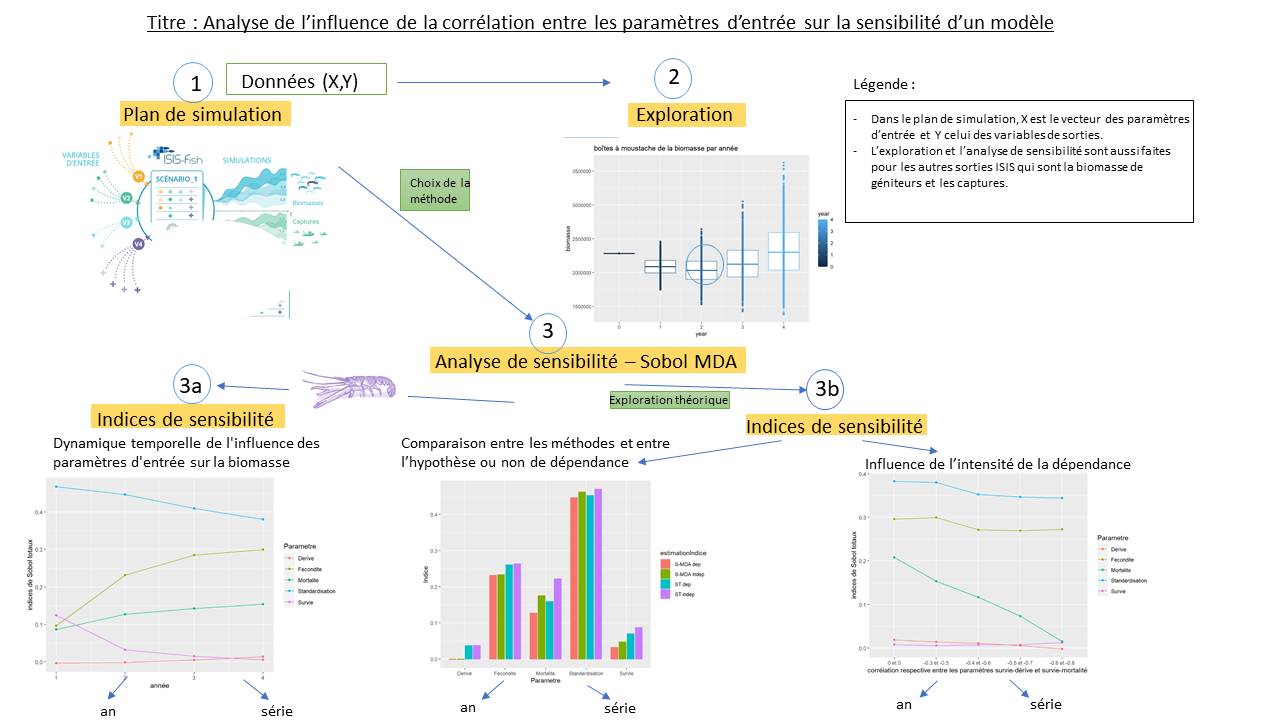
\includegraphics{GraphicalAbstract.png}
\caption{Graphical abstract}
\end{figure}

\newpage

\hypertarget{muxe9thode}{%
\section{Méthode}\label{muxe9thode}}

Dans cette partie nous présentons les randoms forests, la mesure
d'importance Sobol-MDA ainsi que la démarche mise en oeuvre.

\hypertarget{muxe9thodes-utilisuxe9es}{%
\subsection{Méthodes utilisées}\label{muxe9thodes-utilisuxe9es}}

Les random forests sont des algorithmes qui, après avoir été entraînés
sur des données d'entraînement, sont capables de prédire une valeur de
sortie y pour n'importe quelle valeur d'entrée. Les random forests sont
constitués d'arbres de régression si Y est continue ou de classification
si Y est catégorielle, ils sont présentés dans Breiman (2017). Dans
notre cas, le random forest sera composé d'arbres de régression car la
sortie Y de notre modèle est continue. Nous nous baserons sur le livre
de Breiman (2017) pour expliquer en détails la construction de ces
arbres puis nous nous baserons sur les articles de Breiman (2001) et de
Scornet (2023) pour comprendre la construction d'une forêt aléatoire et
l'estimation de son erreur généralisée. Ensuite nous présenterons ranger
(détaillé dans Wright and Ziegler (2015)), une implémentation rapide et
adaptée aux grandes dimensions de random forest utlisée dans Sobol-MDA
(Bénard, Da Veiga, and Scornet (2022)) pour la construction du random
forest. Finalement, nous détaillerons la manière dont Sobol-MDA calcule
les mesures d'importance de chaque covariables ainsi que les hypothèses
et résultats de convergence de cet algorithme.

\hypertarget{arbres-de-ruxe9gression}{%
\subsubsection{Arbres de régression}\label{arbres-de-ruxe9gression}}

Les CART (Classification And Regression Tree décrit dans Breiman (2017)
) sont les composants élémentaires d'une forêt aléatoire. Nous allons
voir dans la suite comment se déroule leur construction. L'algorithme de
construction effectue un partitionnement récursif des données, puis
estime un modèle très simple dans chaque élément de la partition. Un
élément de la partition est appelé feuille de l'arbre. En résumé, le but
est de choisir ``intelligemment'' une caractéristique puis de couper
astucieusement les données selon cette caractéristique de sorte que la
prévision \(y_i\) soit la moyenne des observations dans la feuille. On
recommence ensuite ce processus sur les sous-arbres obtenus jusqu'à
notre critère d'arrêt. Voyons cela en détails.

On considère qu'on a n individus et on note \(X_i\) le vecteur des p
covariables d'entrée, on a alors \(X_{i,k}\) avec \(i \in \{1,...,n\}\)
et \(k \in \{1,...,p\}\). On note \(Y_i\) la variable de sortie à
prédire associée au vecteur d'entrée \(X_i\). L'objectif est de découper
l'espace en J régions \(R_1,..., R_j\) (les feuilles de l'arbre) qui
minimisent :
\[RSS=\sum_{j=1}^{J}{\sum_{i\in R_j}{}}{(y_{i}-\hat{y_j})^2}\]

où \(\hat{y_j}\) est la moyenne des sorties obtenues avec les entrées
situées dans la région \(R_j\) c'est à dire
\(\hat{y_j}=\frac{1}{n_j}\sum_{i\in R_j}y_i\) avec \(n_j\) le nombre
d'observations dans la feuilles \(R_j\). Dans le CART de base on suppose
que \(\hat{y_j}=a\) où a est une constante mais il existe des variantes
de type \(\hat{y_j}=x \beta\).

Pour faire cela, à chaque noeud il faut choisir une variable (i.e une
composante du vecteur X ) selon laquelle on divise les données. On
considère les zones \(R_{-}(k,s)=\{x_i \text{ tel que }x_{i,k}<s\}\) et
\(R_{+}(k,s)=\{x_i\text{ tel que }x_{i,k}\geq s\}\). A chaque étape,
CART choisit la variable j et le seuil s (on a (k,s) \(\in C\)
l'ensemble des coupes possibles dans les données d'un noeud) minimisant
la variance intra-groupe définie comme suit :
\[VI=\frac{1}{n_{noeud}}\sum_{i \text{ tel que } X_i \in R_{-}(j,s)}(y_i-\hat{y}_{R_{-}})^2+\frac{1}{n_{noeud}}\sum_{i \text{ tel que } X_i\in R_{+}(j,s)}(y_i-\hat{y}_{R_{+}})^2\]
où \(n_{noeud}\) est le nombre de données dans le noeud que l'on cherche
à diviser (pour le noeud initial de l'arbre on a donc \(n_{noeud}=n\)).
Minimiser la somme des carrée des résidus revient donc à minimiser
\[RSS=\sum_{j=1}^{J}n_jVj\] où
\(V_j=\frac{1}{n_j}\sum_{i\in R_j}(y_i-\hat{y_j})^2\) est la variance
intra-groupe et \(n_j\) le nombre d'observations dans chaque feuille de
l'arbre.

Dans l'algorithme random forest que nous utilisons, à chaque noeud de
l'arbre, on recherche quelle est la meilleure division non sur toutes
les covariables possibles mais sur un échantillon de m covariables
tirées aléatoirement et sans remplacement. La meilleure division est
sélectionnée uniquement parmi ce m covariables (ce qui présente un gain
de temps considérable pour les problèmes de grandes dimensions). Par
défaut, on prend \(m=\frac{p}{3}\) en régression mais on peut aussi
prendre \(m=\sqrt{p}\) dans les cas de très grandes dimensions.

Concernant l'arrêt de l'algorithme de construction, deux critères sont
principalement utilisés :

\begin{itemize}
\item
  un nombre d'observations q suffisamment petit dans les feuilles
\item
  un critère d'erreur (ici la variance inter-groupe) inférieur à un
  seuil \(\delta\)
\end{itemize}

On peut choisir d'arrêter la récursion lorsque les deux critères sont
vérifiés ou seulement lorsque l'un des deux est vérifié.

\hypertarget{construction-dune-foruxeat-aluxe9atoire}{%
\subsubsection{Construction d'une forêt
aléatoire}\label{construction-dune-foruxeat-aluxe9atoire}}

Une forêt aléatoire n'est rien d'autre qu'un ensemble d'arbres de
décision (dans notre cas d'arbres de régression). Ainsi, avant la
construction de chaque arbre k on tire un échantillon aléatoire
bootstrap \(D_k\) de taille n dans l'échantillon intial D de taille n
lui aussi, c'est-à-dire que l'on tire aléatoirement, uniformément et
avec remise n vecteurs \(x_i\) dans D. Cet échantillon \(D_k\) servira
alors de données d'entraînement pour l'arbre k. Les vecteurs \(x_i\) qui
n'ont pas été tirés (il y en a sûrement grâce au tirage avec remise)
sont gardés de côté et constituent l'échantillon Out Of Bag de cet
arbre. La prédiction par la forêt aléatoire est alors la moyenne des
prédictions de chaque arbre de la forêt.

\hypertarget{calcul-de-lerreur-guxe9nuxe9ralisuxe9e-dune-foruxeat}{%
\subsubsection{Calcul de l'erreur généralisée d'une
forêt}\label{calcul-de-lerreur-guxe9nuxe9ralisuxe9e-dune-foruxeat}}

Lorsque l'on construit une forêt aléatoire il est essentiel de savoir à
quel point les prédictions qu'elle réalise sont précises. Pour cela il
est possible d'estimer son erreur généralisée, ce qui revient en
pratique à calculer le carré de la différence entre les valeurs de
sortie des échatillons OOB et les valeurs de sortie des échantillons OOB
prédites par la forêt et de moyenner le tout. Pour faire cela,
l'algorithme suivant (présenté dans Cutler, Cutler, and Stevens (2012)
et ) peut être utlisé :

Soit \(D_k\) le k-ème échantillon bootstrap et \(\hat{h}_j(x)\) la
prédiction de \(x\) à partir du j-ème arbre, pour \(j = 1, . . . , J\).
Pour \(i = 1\) à \(n\) :

\begin{enumerate}
\def\labelenumi{\arabic{enumi}.}
\item
  Soit \(J_i = \{ j : (x_i, y_i) \notin D_j\}\) et \(|J_i|\) le cardinal
  de \(J_i\).
\item
  Définissons la prédiction hors sac à \(x_i\) comme suit :

  \begin{itemize}
  \tightlist
  \item
    \(\hat{f}_{oob}(x_i) = \frac{1}{|J_i|} \sum_{j \in J_i} \hat{h}_j(x_i)\)
    pour la régression
  \end{itemize}
\end{enumerate}

L'erreur de généralisation est généralement estimée en utilisant
l'erreur quadratique moyenne (MSE) hors sac suivante :

\[
\text{MSE}_{oob} = \frac{1}{n} \sum_{i=1}^{n} (y_i - \hat{f}_{oob}(x_i))^2
\]

En résumé, pour chaque vecteur \(x_i\) de l'ensemble d'entraînement
initial D, on calcule sa prédiction par chacun des arbres k dont il n'a
pas fait partie de l'ensemble d'entraînement \(D_k\) et on moyenne ces
prédictions pour avoir sa prédiction ``par la forêt'' (même si dans ce
cas on ne l'a pas fait passer par tous les arbres). Ensuite, pour
obtenir l'estimation généralisée de la forêt on fait la moyenne des
différences au carré de la prévision de chaque \(x_i\) et de sa valeur
de sortie présente dans l'échantillon d'entraînement D.

\hypertarget{mesure-dimportance-des-variables-gruxe2ce-uxe0-lalgorithme-sobol-mda}{%
\subsubsection{Mesure d'importance des variables grâce à l'algorithme
Sobol-MDA}\label{mesure-dimportance-des-variables-gruxe2ce-uxe0-lalgorithme-sobol-mda}}

Un des problèmes majeurs des random forests réside dans le fait que
leurs propriétés mathématiques restent toujours un peu ``magiques'', ce
qui rend leur interprétabilité plus compliquée. Les personnes désireuses
de se pencher d'avantage sur les forces à l'oeuvre derrière le processus
de prédiction se sont alors principalement tournées vers l'importance
des variables, une mesure de l'influence de chaque variable d'entrée
dans la prédiction de la sortie. Dans l'article initial de Breiman
(2001) sur les random forests, deux mesures d'importance sont présentées
: la diminution moyenne de l'impureté (MDI, ou Gini importance, voir
Breiman (2002) ) qui somme les diminutions pondérées de l'impureté sur
tous les noeuds qui se divisent selon une covariable donnée, et la
diminution moyenne de la précision (MDA, voir Breiman (2001)) qui
permuttent les valeurs d'entrée d'une certaine variable dans les données
du test et calcule la différence entre l'erreur sur l'ensemble test
permutté et l'ensemble test original. L'un des grands avantages du MDI
et du MDA réside dans leur capacité à prendre en compte l'intéraction
entre les covariables mais d'un autre côté ils sont incapables de
déterminer la partie de l'effet marginal d'une covariable donnée ((voir
Wright, Ziegler, and König (2016)). Par ailleurs, MDA et MDI présentent
tous les deux des biais non négligeables dans le cas de variables
corrélés. Une version modifiée du MDA, nommée Sobol-MDA et expliquée
dans Bénard, Da Veiga, and Scornet (2022), a ainsi été développée pour
être capable de donner des résultats pertinents même dans des cas de
corrélations entre les variables. Nous avons donc choisi d'utiliser
Sobol-MDA pour évaluer la sensibilité de notre modèle.

Après avoir brièvement expliqué le fonctionnement du MDA, nous nous
intéressons plus en détails à l'algorithme Sobol-MDA et nous verrons
certains résultats de convergence de celui-ci.

\hypertarget{pruxe9sentation-et-limites-du-mda}{%
\paragraph{Présentation et limites du
MDA}\label{pruxe9sentation-et-limites-du-mda}}

Le MDA, mesure de la diminution de la précision en français, a été
initialement introduit pas Breiman dans son article Breiman (2001). Il
repose sur le fonctionnement suivant : les valeurs d'une covariable
spécifique sont permutées pour casser sa relation avec la variable de
sortie. La précision prédictive est alors calculée pour cet ensemble de
donées permutées. La différence entre la précision de l'ensemble dégradé
et la précision de l'ensemble intial est alors calculée, cette
différence donne la mesure d'importance de la covariable pour laquelle
on a permuté les valeurs. Une grande diminution de la précision signifie
que la variable considérée a une grande influence dans le mécanisme de
prédiction. Bien que cette mesure soit très utilisée en pratique, on ne
sait que très peu de choses sur ces propriétés statistiques. Sa
convergence vers les indices de Sobol totaux n'a pas pu être prouvée et
de nombreuses études empiriques ont montré que, lorsque les covariables
sont dépendantes, le MDA ne détecte pas certaines variables influentes.
Pour tenter d'y remédier, Williamson et al. (2023) proposent de mesurer
la diminution de la précision entre la forêt originale et une forêt
entraînée sans l'une des covariables. Néanmoins, comme il faut
réentraîner la forêt et calculer sa précision autant de fois qu'il y a
de covariables, cette méthode a un coût de calcul très élevé et n'est
pas adaptée aux grandes dimensions.

\hypertarget{sobol-mda}{%
\paragraph{Sobol-MDA}\label{sobol-mda}}

La mesure d'importance Sobol-MDA propose de mimer l'entraînement d'une
forêt sans l'une des covariables sans avoir besoin de réentraîner une
forêt. Expliquons cela plus clairement.

Le Sobol-MDA (Bénard, Da Veiga, and Scornet (2022)), une amélioration de
la méthode MDA, a été introduit pour estimer les indices de Sobol totaux
même lorsque les covariables (X) sont dépendantes. Cette méthode vise à
estimer les indices de Sobol totaux. Les indices de Sobol totaux
correspondent à la proportion de la variance expliquée de la réponse
perdue lorsqu'une des covariables est retirée du modèle (voir l'annexe
sur les indices de Sobol pour plus de détails). L'indice de sensibilité
total de l'entrée \(X_i\) est défini comme la somme des indices associés
à l'effet principal de \(X_i\) et à toutes les interactions entre
\(X_i\) et d'autres entrées (voir figure 2).

\begin{figure}
\centering
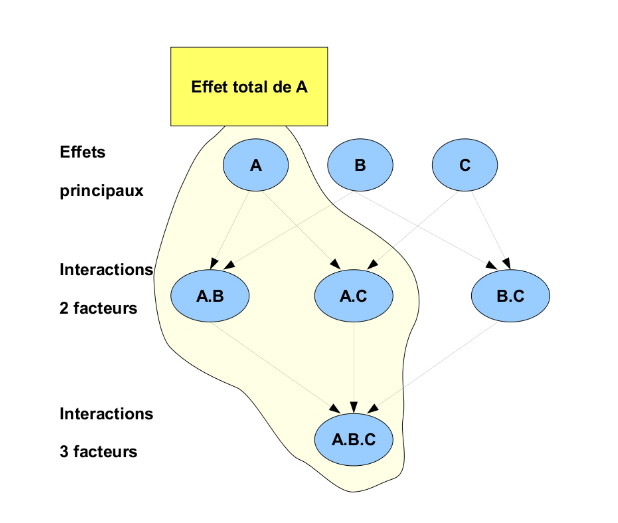
\includegraphics{effetsTotaux.png}
\caption{Termes factoriels composant l'indice de sensibilité total de
l'entrée A}
\end{figure}

Pour le dire d'une troisième façon, la sensibilité totale mesure donc la
variance moyenne (normalisée) de Y quand toutes les entrées sauf \(X_i\)
sont fixées. Lorsque l'on souhaite effectuer un factor fixing,
c'est-à-dire choisir les entrées à fixer, on utilise principalement les
indices totaux. Les indices de sensibilité totaux très faibles
correspondent en effet aux entrées que l'on peut fixer arbitrairement
sans modifier sensiblement le comportement du modèle.

\hypertarget{algorithme}{%
\paragraph{algorithme}\label{algorithme}}

Pour retirer une variable j du processus de prédiction de l'arbre on
procède comme suit. La partition de l'espace de covariables obtenue avec
les feuilles terminales de l'arbre d'origine est projetée selon la
j-ième direction et les sorties des cellules de cette nouvelle partition
projetée sont recalculées avec les données d'entraînement. Ce procédé
permet de retirer la variable j du processus de prédiction de l'arbre.
Ensuite, il est possible de calculer la précision de l'estimation de la
forêt projetée grâce aux échantillons OOB, de soustraire cette précision
de la précision initiale et de normaliser la différence obtenue par
\(V [Y ]\) pour obtenir le Sobol-MDA pour \(X_j\).

En pratique, les données d'entraînement et les échantillons OOB de
l'arbre sont mis dans l'arbre et envoyés à droite et à gauche du noeud
si celui-ci fait une division sur la covariable j. A la fin, chaque
donnée peut donc se retrouver dans plusieurs feuille terminales. Pour
chaque donnée OOB, la prédiction associée est donc la moyenne des
sorties des données d'entraînement qui sont tombées sur les mêmes
feuilles terminales que la donnée OOB. En d'autres termes on calcule
l'intersection entre les feuilles terminales où est tombée la donnée OOB
et les feuilles terminales où sont tombées les données d'entraînement.
Cette intersection donne la cellule projetée. Ce mécanisme est
équivalent à projeter la partition de l'arbre sur le sous-espace
engendré par \(X^{(-j)}\).

Ecrivons cela plus formellement.

On note \(\Theta\) le vecteur qui contient les indices des vecteurs de
l'échantillon initial utilisé pour l'entraînement de l'arbre auquel il
est associé et on note \(m_n(x,\Theta)\) l'estimation de la valeur de la
sortie de x par un arbre entraîner avec un échantillon indiqué par
\(\Theta\) , Sobol-MDA prédit donc
\(m^{(-j)}(X^{(-j)})=E[m(X)|X^{(-j)}]\).

On note \(A_n(X,\Theta)\) la cellule de la partition de l'arbre
d'origine où X tombe et on note \(A_n^{(-j)}(X^{(-j)},\Theta)\) la
cellule associé de la partition projetée. On note l'estimation par
l'arbre projeté associé \(m_n^{(-j)}(X^{(-j)},\Theta)\) et l'estimation
par la forêt projeté associée
\(m_{M,n}^{(-j,OOB)}(X_i^{(-j)},\Theta_{(M)})\). Ces estimations sont
définies de la manière suivante :

\[m_n^{(-j)}(X^{(-j)},\Theta)=\frac{\sum_{i=1}^{a_n} Y_i 1_{X_i \in A_n^{(-j)}(X^{(-j)},\Theta)}}{\sum_{i=1}^{a_n} 1_{X_i \in A_n^{(-j)}(X^{(-j)},\Theta)}}\]
\[m_{M,n}^{(-j,OOB)}(X_i^{(-j)},\Theta_{(M)})=\frac{1}{|\Lambda_{n,i}|} \sum_{l \in \Lambda_{n,i}} m^{(-j)}_{n}(X^{(-j)}_i, \Theta_l)1_{|\Lambda_{n,i}|>0}
\]

L'indice de Sobol-MDA est donné par la différence normalisée de l'erreur
carrée (calculée grâce aux OOB) de la forêt projetée et l'erreur carrée
(calculée grâce aux OOB) de la forêt initial, Sobol-MDA est donc défini
de la manière suivante :

\[\widehat{S-MDA}_{M,n}(X^{(j)})=\frac{1}{\hat{\sigma}^2_Y}\frac{1}{n}\sum^{n}_{i=1}\{Y_i-m_{M,n}^{(-j,OOB)}(X_i^{(-j)},\Theta_{(M)})\}^2\]
\[-\{Y_i-m_{M,n}^{(OOB)}(X_i,\Theta_{(M)})\}^2\] où
\(\hat{\sigma}^2_Y=\frac{1}{n-1}\sum^{n}_{i=1}(Y_i-\bar{Y})^2\) est la
variance standard estimée de la réponse Y.

\hypertarget{convergence}{%
\paragraph{convergence}\label{convergence}}

Dans l'article Bénard, Da Veiga, and Scornet (2022), , sous certaines
hypothèses sur la construction du random-forest faciles à mettre en
place, la convergence des indices Sobol-MDA vers les indices de Sobol
totaux lorsque le nombre d'échantillons augmente a été prouvé. Nous
présentons ici l'idée générale de la preuve.

L'indice de Sobol total \(S_j^T=\frac{E[Var(G(X)|X^{(-j)})]}{VarG(X)}\),
s'écrit, dans le cas du random forest, en remplaçant G(X) par
l'estimation obtenue par la forêt, l'indice de Sobol total s'écrit donc
\(S_j^T=\frac{E[Var(m(X)|X^{(-j)})]}{Var[m(X)]}=\frac{E[(m(X)-E[m(X)|X^{(-j)}])^2]}{Var(m(X))}\).
On cherche donc à montrer que
\[\widehat{S-MDA}_{M,n}(X^{j})\overset{p}{\longrightarrow}S_j^T\]

Pour cela, on majore
\(E[\widehat{S-MDA}_{M,n}(X^{j})\sigma_Y^2-E[(m(X)-E[m(X)|X^{(-j)}])^2]]\)
par une expression dépendant de n en faisant une décomposition sur
laquelle on applique l'inégalité triangulaire. On obtient alors
\[\widehat{S-MDA}_{M,n}(X^{j})\sigma_Y^2\overset{p}{\longrightarrow}E[(m(X)-E[m(X)|X^{(-j)}])^2]\]

Ensuite l'indice de Sobol-MDA est normalisé par la variance standard
estimée \(\sigma_Y^2\) de la sortie Y qui est convergente par la loi des
grands nombres. Grâce au ``mapping theorem'' on a
\[\frac{1}{\hat\sigma_Y^2}\overset{p}{\longrightarrow}\frac{1}{V[Y]}\]
Sobol-MDA est donc le produit de deux quantités aléatoires qui converge
en probabilité donc on obtient bien
\[\widehat{S-MDA}_{M,n}(X^{j})\overset{p}{\longrightarrow}\frac{E[(m(X)-E[m(X)|X^{(-j)}])^2]}{V[Y]}=S_j^T\]

\hypertarget{avantages}{%
\paragraph{avantages}\label{avantages}}

L'approche de Williamson et al. (2023), consitant à réentraîner une
forêt sans l'une des covariables, permet elle aussi d'approximer les
indices de Sobol totaux. Néanmoins, l'avantage de l'approche Sobol-MDA
est qu'elle nécessite seulement de faire des prédiction supplémentaires
avec la forêt, ce qui est plus rapide que le réentraînement d'une forêt.
L'algorithme de Williamson et al. (2023) a une complexité en
\(O\{Mp^2nlog^2(n)\}\) qui est quadratique avec les dimensions et
l'algorithme Sobol-MDA a une complexité en \(O\{Mnlog^3(n)\}\) ce qui
est un grand avantage lorsque l'on travaille avec un grand nombre de
varaibles d'entrée.

Concernant l'analyse des résultats, nous avons tout d'abord exploré les
sorties du modèles pour comprendre leur dynamique. Nous avons étudié la
dynamique temporelle des sorties, la propagation de l'incertitude
d'entrée sur les sorties ainsi que la variabilité des sorties lorsqu'un
seul des paramètres varie et que les autres sont fixés. Nous avons
ensuite pu construit 2 métamodèles random forests en utilisant ranger
(Wright and Ziegler (2015)), l'un lorsque les paramètres sont dépendants
et l'autre losrque les paramètres sont indépendants. Nous avons ensuite
estimé les indices de Sobol totaux sur les randoms forests en utilisant
la méthode ``Sobol-MDA''. D'une part nous avons pu voir les paramètres
qui inluent le plus sur les sorties et d'autre part nous avons pu
comparer les valeurs des indices pour les paramètres dépendants et
indépendants ainsi que les valeurs des indices obtenues selon les
différentes méthodes de calcul (Sobol-MDA ou méthode classique du
package sensitivity). Finalement, pour comprendre comment l'intensité de
la dépendance influe sur l'analyse de sensibilité, nous avons construit
des random forests avec des jeux de données dont les paramètres étaient
de plus en plus corrélés. Nous avons calculé les indices de Sobol-MDA
sur ces random forest et tracer l'évolution des valeurs des indices en
fonction de la corrélation entre les paramètres d'entrée.

\hypertarget{duxe9marche-mise-en-oeuvre}{%
\subsection{Démarche mise en oeuvre}\label{duxe9marche-mise-en-oeuvre}}

Pour réaliser cette étude, nous construisons plusieurs fichiers csv
contenant les combinaisons des valeurs des paramètres d'entrée, et plus
précisément un fichier avec des paramètres d'entrée suivant une
distribution avec une hypothèse d'indépendance, d'autres avec
différentes hypothèses de dépendance, et d'autres avec un paramètre fixe
et 4 qui varient. Pour chaque fichier nous avons faits des simulations
avec ISIS pour chacunes des combinaisons de paramètres d'entrée. Nous
avons ensuite construits plusieurs fichiers rds contenant les valeurs
des paramètres associés aux valeurs des sorties du modèle ISIS.

Concernant l'analyse des résultats, nous avons tout d'abord exploré les
sorties du modèles pour comprendre leur dynamique. Nous avons étudié la
dynamique temporelle des sorties, la propagation de l'incertitude
d'entrée sur les sorties ainsi que la variabilité des sorties lorsqu'un
seul des paramètres varie et que les autres sont fixés. Pour chaque
export du modèle (biomasse, biomasse de géniteurs et captures de pêche),
nous avons ensuite construit 2 métamodèles random forests en utilisant
ranger (Wright and Ziegler (2015)), l'un lorsque les paramètres sont
dépendants et l'autre lorsque les paramètres sont indépendants. Nous
avons ensuite estimé les indices de Sobol totaux sur les randoms forests
en utilisant la méthode ``Sobol-MDA''. D'une part nous avons pu voir les
paramètres qui inluent le plus sur les sorties et d'autre part nous
avons pu comparer les valeurs des indices pour les paramètres dépendants
et indépendants ainsi que les valeurs des indices obtenues selon les
différentes méthodes de calcul (Sobol-MDA ou méthode classique
shapleysobol\_knn() du package sensitivity). Finalement, pour comprendre
comment l'intensité de la dépendance influe sur l'analyse de
sensibilité, nous avons construit des random forests avec des jeux de
données dont les paramètres étaient de plus en plus corrélés. Nous avons
calculé les indices de Sobol-MDA sur ces random forest et tracer
l'évolution des valeurs des indices en fonction de la corrélation entre
les paramètres d'entrée.

\hypertarget{donnuxe9es}{%
\section{Données}\label{donnuxe9es}}

L'un des objectifs de cette étude étant d'évaluer la sensibité des
sorties du modèle ISIS-Fish à certains paramètres d'entrée, nous allons
dans ce chapitre présenter plus en détails le simulateur ISIS-Fish
(voire Mahévas and Pelletier (2004)). Ensuite nous nous intéressons à la
pêcherie langoustinière et aux paramètres d'entrée que nous allons faire
varier pour évaluer la sensibilité. Finalement nous expliquerons le plan
de simulations mis en place.

\hypertarget{pruxe9sentation-disis-fish}{%
\subsection{Présentation d'ISIS-Fish}\label{pruxe9sentation-disis-fish}}

ISIS-Fish (Integration of Spatial Information and Simulation for
Fisheries) est un simulateur des dynamiques de pêche. Il peut aider les
pêcheurs, les managers, les entreprises et les scientifiques dans leur
recherche de la meilleure gestion écosystémique spatialisée des pêches.
Mais comment marche ce modèle mécanistique ? Tout d'abord, il faut avoir
en tête que ce modèle est composé de trois sous-modèles qui
intéragissent à travers le temps et l'espace. Précisons que le pas de
temps est le mois et qu'un maillage de l'espace est réalisé pour obtenir
des zones. Parmi les sous-modèles on trouve la modélisation du
management, de l'activité de pêche et des dynamiques des populations de
poissons. Leurs intéarctions sont représentées dans la Figure 3.

\begin{figure}
\centering
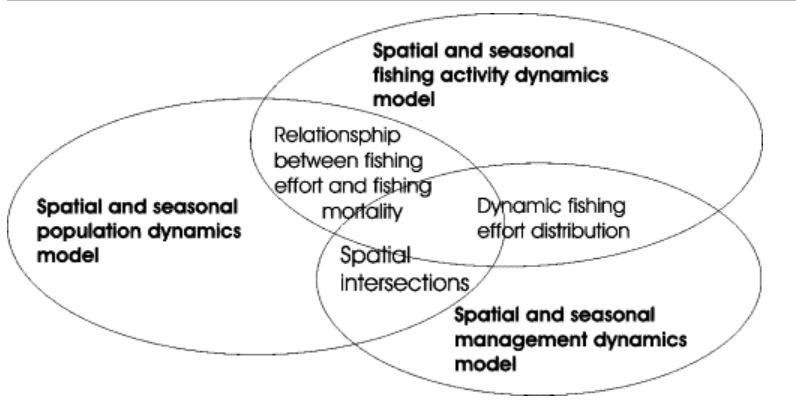
\includegraphics{3sousModeles.png}
\caption{Une vue générale du modèle de pêcherie spatiale mixte décomposé
en trois sous-modèles interagissant à travers le temps et l'espace. Les
sous-modèles interagissent via une intersection spatiale et temporelle.
(trouvé dans Mahévas and Pelletier (2004))}
\end{figure}

La composante ``management'' simule les règles qui s'appliquent sur la
pêche (mesures de sélectivité, TCA, zones protégées, saisons interdites,
etc). La composante ``populations de poissons'' simule le cycle de vie
des poissons. Chaque mois les poissons grandissent, migrent, se
reproduisent, et certains meurent de causes naturelles (voire Figure 4).
Pour chaque mois, une carte de l'abondance des poissons par zone est
produite par ISIS.

\begin{figure}
\centering
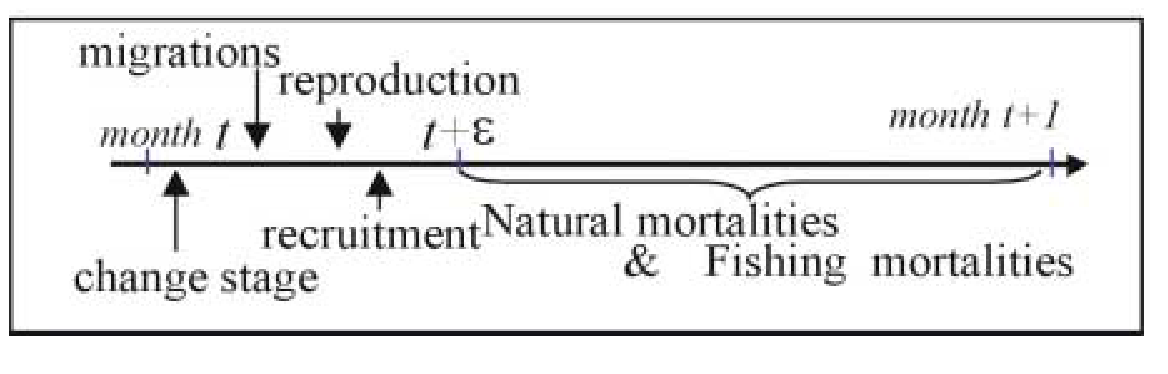
\includegraphics{processusPopModele.png}
\caption{Chronologie des processus considérés dans le modèle de
population, fishing mortalities provient de l'intéraction entre la
composante ``dynamique des populations'' et ``dynamique des pêches''}
\end{figure}

La composante ``dynamique des pêches'' simule l'exploitation des
ressources halieutiques. Celle-ci est quantifiée par l'effort de pêche,
qui dépend des engins de pêche utilisés et de la durée passée à pêcher.
Les navires de pêche ne sont pas représentés individuellement mais ils
sont organisés en flottes rattachées à des zones de pêche selon la durée
passée en mer et selon leurs caractéristiaues techniques. Pour chaque
flotte, des stratégies décrivent la distribution de l'effort de pêche en
fonction des métiers et des mois. Les statégies peuvent changer en
fonction des mesures de management, de l'abondance des populations, du
prix de l'essence et du prix de vente des poissons. Chaque mois, la
carte (toujours à l'échelle des zones) de l'effort de pêche est alors
mise à jour.

A la fin de chaque mois, ISIS-Fish superpose la carte de l'effort de
pêche sur celle de l'abondance des populations. Pour les espèces que
l'on considère ``immobiles'', les captures par la flotte sont alors
calculées sur les zones d'intersection (car on a donc sur ces zones des
poissons et des pêcheurs). Pour les espèces qui se déplacent, les
captures ne sont pas seulement calculées sur le nombre d'animaux marins
présents dans la zone d'intersection mais aussi sur ceux des zones
adjacentes qui passeront probablement par les zones d'intersection
durant la durée de la pêche. En fonction des stratégies mises en place
et de la réglementation, les pêcheurs décident des poissons à garder et
de ceux à remettre à l'eau, on représente cela dans le modèle avec la
probabilité de survie après relâchement.

Avant d'utiliser ISIS-Fish comme un outil d'aide à la prise de décision,
les valeurs des paramètres doivent être sélectionnées pour représenter
au mieux la pêcherie étudiée. Pour cela, des données de pêche et des
données d'études sont utilisées et des hypothèses sont faites dans le
cas d'informations manquantes. Pour valider ou invalider les paramètres,
on compare les résultats du simulateur avec les données sur la situation
passée de la pêcherie étudiée.

Après validation des paramètres on peut simuler différents scénarios de
management pour voir lequel conviendrait le mieux. Par exemple, on peut
estimer le poids des captures de pêche dans 5 ans dans le cadre de mise
en place d'une zone de pêche protégée. Des simulations sont alors faites
avec des valeurs de paramètres prises aléatoirement dans leur intervalle
de confiance. On obtient alors non pas une valeur de sortie mais un
intervalle de valeurs de sortie. On prend ainsi en compte la propagation
de l'incertitude d'entrée dans la sortie. Un des objectif est de réduire
les incertitudes en entrée pour ainsi réduire l'incertitude en sortie.
L'analyse d'incertitude est très utiles dans le sens où, en nous
fournissant les paramètres d'entrée qui augmente le plus la variance de
la sortie, elle nous permet de connaître les paramètres pour lesquels on
doit chercher en prorité à réduire l'incertitude.

\hypertarget{pruxe9cisions-sur-la-puxeacherie-langoustinuxe8re}{%
\subsection{Précisions sur la pêcherie
langoustinère}\label{pruxe9cisions-sur-la-puxeacherie-langoustinuxe8re}}

La pêcherie langoustinière étudiée ici est inspirée de la pêcherie de la
grande vasière dans le golfe de Gascogne paramétrée avec ISIS-Fish. La
paramétrisation a été simplifiée pour faciliter l'utilisation et la
compréhension de ce modèle.

Le cycle de vie de la langoustine est décrit dans le modèle au travers
de 10 classes d'âge qui se distribuent spatialement sur 9 rectangles de
taille 1 degré en longitude et 0.5 degré en latitude. Chaque classe
d'âge se caractérise par une largeur moyenne de la carapace de la tête
(longueur céphalothoracique) qui permet de décrire l'interdiction de
débarquer des langoustines dont la carapace de la tête est plus petite
que 20 mm (réglementation de la taille minimale de débarquement). Si une
langoustine trop petite est capturée, elle est rejetée dans la mer avec
une chance de survie (proportion de survie). Le renouvellement annuel
des langous- tines juvéniles est dépendant de la quantité de
langoustines en âge de se reproduire (relation stock-recrute- ment de
Beverton et Holt). Dans cette description, on fait l'hypothèse qu'il n'y
a pas de dispersion des larves à l'extérieur des 9 rectangles ni entre
les rectangles. A chaque mois de l'année, le modèle décrit la carte du
nombre de langoustines par classe d'âge (abondance ou biomasse en
poids). Les langoustines sont capturées par plusieurs groupes de bateaux
de pêche (chalutiers) qui diffèrent par leur port d'attache, leur
longueur, les espèces ciblées (métiers : langoustiniers, poissons
benthiques, poissons démersaux) et leurs pratiques annuelles des métiers
(stratégies). Le temps passé à pêcher (effort de pêche) est spatialisé
et se distribue différemment selon les métiers et les saisons dans les 9
rectangles. Selon le métier, cet effort de pêche est plus ou moins
efficace pour capturer des langoustines et l'efficacité de pêche change
au cours du temps (dérive d'efficacité de pêche). A chaque mois de
l'année, en multipliant l'effort de pêche par un facteur appelé
capturabilité, le modèle calcule une carte de la mortalité par pêche des
langoustines pour chaque métier. Chaque mois, sur la période de 5 ans
simulée, le modèle prédit les captures, la biomasse et la biomasse
féconde de langoustine par rectangle en superposant les cartes de
mortalité par pêche des métiers et la carte d'abondance des
langoustines. Pour simplifier les exports des résultats du modèles, on a
choisi de sommer les résultats sur les zones et sur les mois. On obtient
ainsi la biomasse, la biomasse féconde et les captures de pêche (en
tonnes) sur la zone de présence totale des langoustines au début du mois
de janvier pour les 5 années suivantes.

\hypertarget{paramuxe8tres-en-entruxe9e}{%
\subsection{Paramètres en entrée}\label{paramuxe8tres-en-entruxe9e}}

\hypertarget{choix-des-paramuxe8tres-incertains}{%
\subsubsection{Choix des paramètres
incertains}\label{choix-des-paramuxe8tres-incertains}}

Dans cette étude, nous nous sommes concentrées sur 5 paramètres
incertains :

\begin{itemize}
\item
  la proportion de survie : pourcentage de survie des captures non
  débarquées pour des raisons diverses (taille illégale, poisson
  endommagé, absence de marché ou dépassement des quotas).
\item
  la dérive d'efficacité de pêche : coefficient d'évolution annuelle de
  l'efficacité de pêche.
\item
  le facteur de standardisation des engins : coefficient de
  standardisation d'une heure de pêche entre différents engins.
\item
  la mortalité naturelle : taux de mortalité naturelle des langoustines
  selon la classe d'âge
\item
  la fécondité : taux de fécondité (nombre d'oeufs ou de juvéniles) des
  langoustines selon la classe d'âge
\end{itemize}

Chacun de ces paramètres a une valeur de référence et un intervalle
d'incertitude autour de cette valeur de reference (voir figure 5). Dans
cette étude on fait l'hypothèse que toutes les valeurs possibles de cet
intervalle ont la même probabilité de se réaliser (distribution
uniforme).

\begin{figure}
\centering
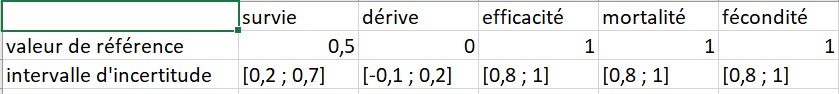
\includegraphics{tabParam.png}
\caption{Tableau de la valeur de référence ainsi que l'intervalle
d'incertitude des paramètres}
\end{figure}

\hypertarget{distributions-des-valeurs-dentruxe9e}{%
\subsubsection{Distributions des valeurs
d'entrée}\label{distributions-des-valeurs-dentruxe9e}}

On peut concevoir que plus le taux de mortalité naturelle des
langoustines est élevé, plus les langoustines sont fragiles et plus
elles ont de chances de mourrir après avoir été relâchées par les
pêcheurs. C'est pourquoi nous avons simulé une hypothèse de dépendance
(corrélation négative) entre les paramètre ``Mortalité et survie''. De
plus, on peut supposer que plus la dérive d'efficacité de pêche est
importante, plus les quantités de langoustines pêchées augmente, plus
les pêcheurs mettent de temps à trier celles à relâcher et plus elles
sont serrées dans les filets et ainsi plus la proportion de survie après
relâchement diminue. C'est pourquoi nous avons simulé une hypothèse de
dépendance (corrélation négative) entre les paramètre ``Dérive et
Survie''. Voici la distribution des valeurs de nos paramètres d'entrée
dans le cas où on a supposé une dépendance.

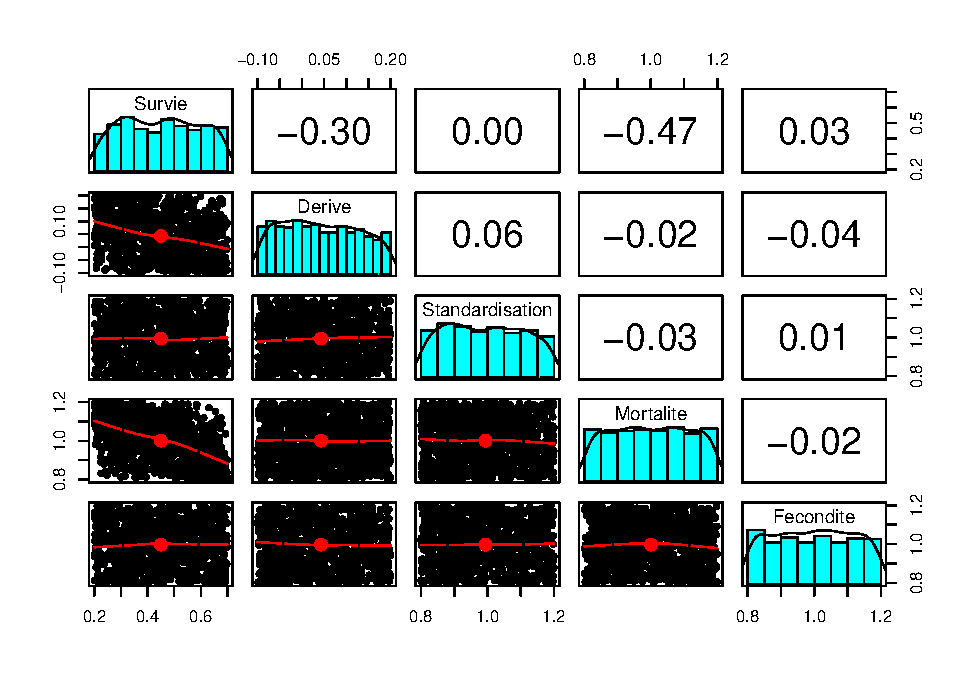
\includegraphics{rapport_files/figure-latex/acx-1.pdf}

\hypertarget{plan-de-simulation}{%
\subsection{Plan de simulation}\label{plan-de-simulation}}

En vue d'étudier la variabilité des sorties lorsqu'un seul des
paramètres varie et que les autres sont fixés nous faisons 50
simulations en faisant varier un seul paramètre. Nous répétons
l'opération pour chaque paramètre. Pour obtenir les données
d'entraînement du random forest et estimer les indices de Sobol- MDA,
nous faisons 1000 simulations avec des valeurs de paramètres tirées
aléatoirement dans leur intervalle respectif, avec ou sans hypothèse de
dépendance suivant le cas. Voici un exemple de fichier de données
utilisé pour la construction des random forests et l'analyse. Ce fichier
contient les combinaisons des paramètres d'entrée, les résultats
associés et ce pour chaque année (voir figure 6).

\begin{figure}
\centering
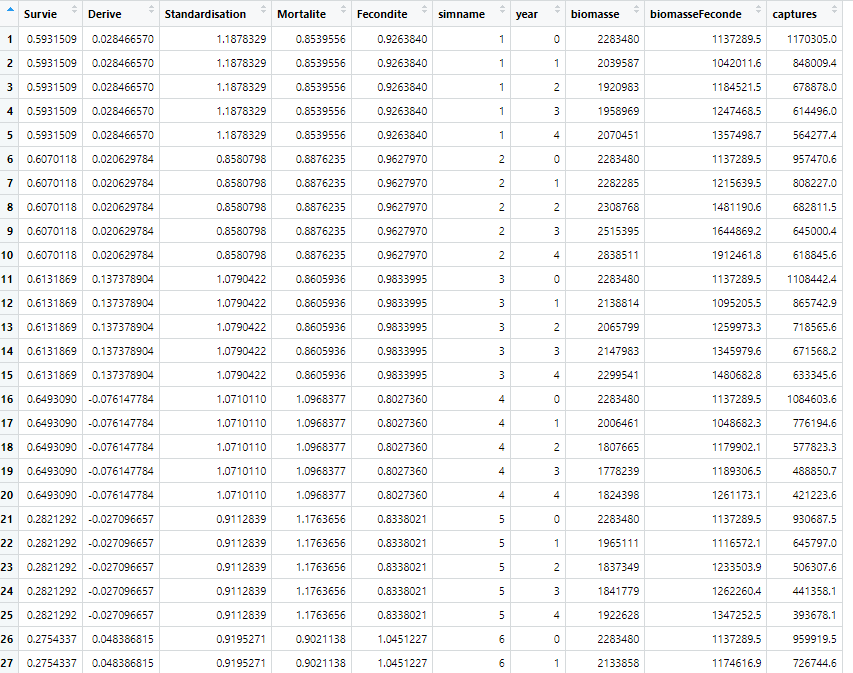
\includegraphics{exDonnees.png}
\caption{Exemple d'un fichier de données utilisé dans notre étude''}
\end{figure}

\newpage

\hypertarget{ruxe9sutats}{%
\section{Résutats}\label{ruxe9sutats}}

\hypertarget{exploration-des-sorties-isis}{%
\subsection{Exploration des sorties
ISIS}\label{exploration-des-sorties-isis}}

Dans cette partie, nous étudions la dynamique temporelle des sorties
d'ISIS, la variabilité des sorties lorsqu'un seul des paramètres varie
et que les autres sont fixés ainsi que la propagation de l'incertitude
d'entrée sur les sorties (par année ainsi que sa série temporelle).

\hypertarget{quelle-est-la-dynamique-temporelle-des-sorties-lorsque-les-entruxe9es-sont-mises-uxe0-leur-valeur-de-ruxe9fuxe9rence}{%
\subsubsection{Quelle est la dynamique temporelle des sorties lorsque
les entrées sont mises à leur valeur de référence
?}\label{quelle-est-la-dynamique-temporelle-des-sorties-lorsque-les-entruxe9es-sont-mises-uxe0-leur-valeur-de-ruxe9fuxe9rence}}

\hypertarget{biomasse}{%
\paragraph{Biomasse}\label{biomasse}}

La biomasse varie entre 2 350 000 et 2 100 000 tonnes, ce qui ne
présente pas un intervalle très large. Ceci est plutôt normal car les
paramètres sont mis à leurs valeurs de référence.

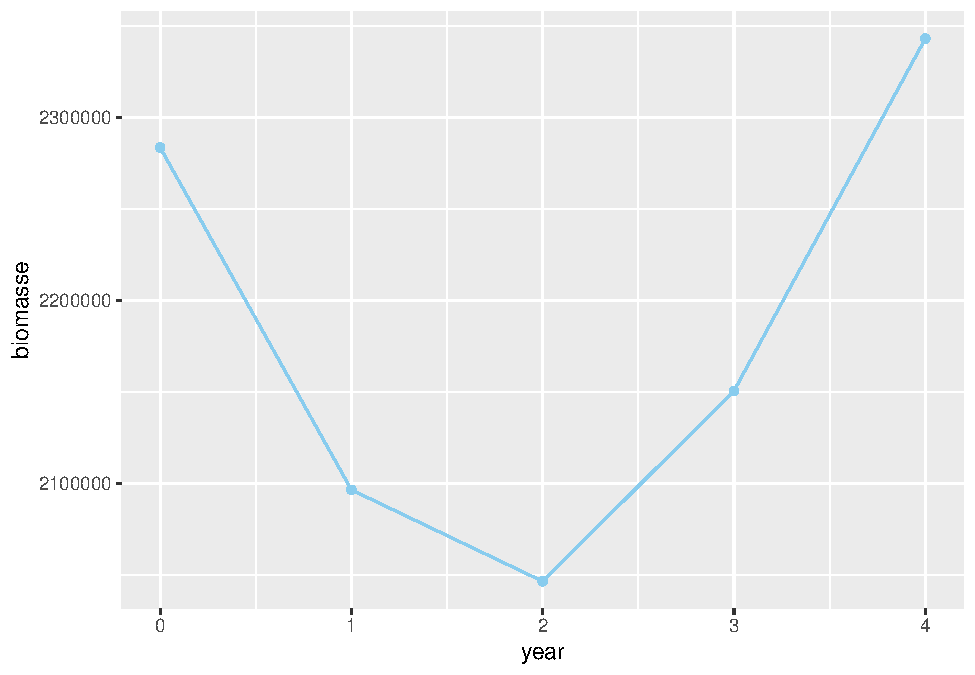
\includegraphics{rapport_files/figure-latex/ref-1.pdf}

\hypertarget{biomasse-fuxe9conde}{%
\paragraph{Biomasse féconde}\label{biomasse-fuxe9conde}}

On remarque que la biomasse féconde n'a pas la même diminution que la
biomasse entre l'année 0 et l'année 2. On peut supposer que des
langoustines sont passées de non fécondes à fécondes entre ces années ce
qui a compensé les pertes.

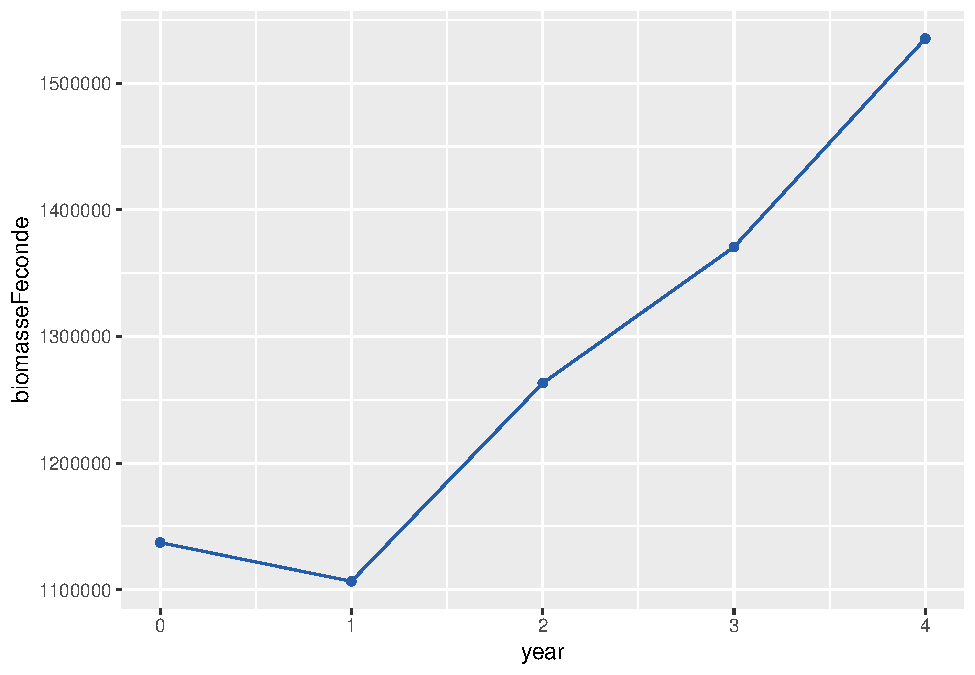
\includegraphics{rapport_files/figure-latex/refbf-1.pdf}

\hypertarget{poids-des-captures-de-puxeache}{%
\paragraph{Poids des captures de
pêche}\label{poids-des-captures-de-puxeache}}

Les captures de pêche diminuent jusqu'à atteindre un plateau. Ceci peut
s'expliquer par le fait que les effectifs initiaux comportaient beaucoup
de langoustines de tailles suffisantes pour être pêchées. Ensuite, cela
commence à s'équilibrer avec les paramètres de référence pour revenir à
une distribution plus classique.

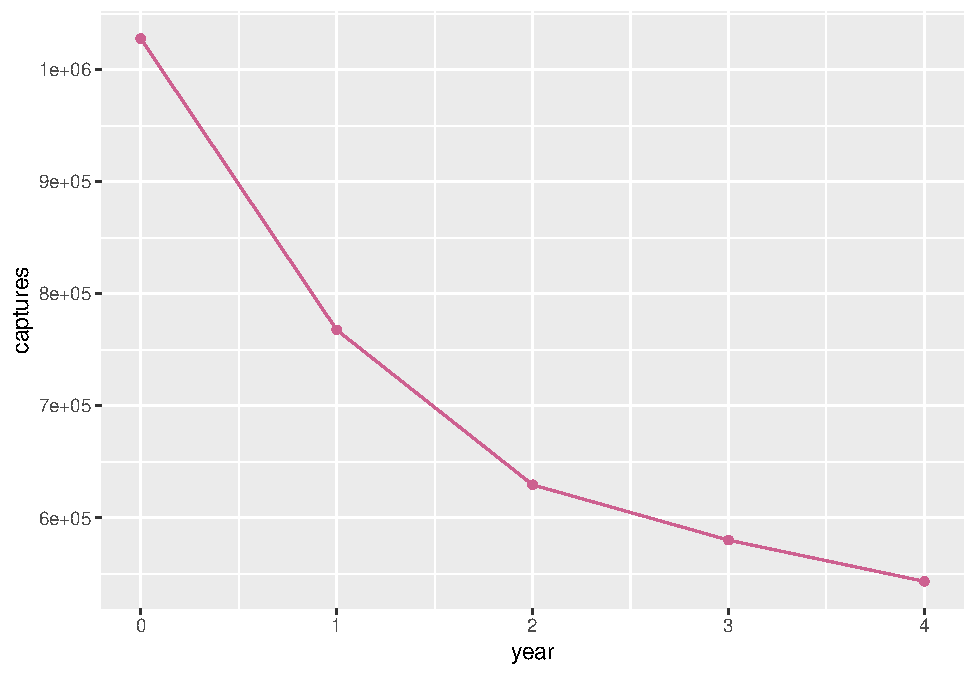
\includegraphics{rapport_files/figure-latex/refc-1.pdf}

\hypertarget{de-quelle-maniuxe8re-varient-les-sorties-lorsquun-seul-des-paramuxe8tres-varie-et-que-les-autres-sont-fixuxe9s-uxe0-leur-valeur-de-ruxe9fuxe9rence}{%
\subsubsection{De quelle manière varient les sorties lorsqu'un seul des
paramètres varie et que les autres sont fixés à leur valeur de référence
?}\label{de-quelle-maniuxe8re-varient-les-sorties-lorsquun-seul-des-paramuxe8tres-varie-et-que-les-autres-sont-fixuxe9s-uxe0-leur-valeur-de-ruxe9fuxe9rence}}

\hypertarget{survie}{%
\paragraph{Survie}\label{survie}}

Etudions les variations des sorties lorsque l'on fait varier la
proportion de survie après relâchement.

\hypertarget{biomasse-1}{%
\subparagraph{Biomasse}\label{biomasse-1}}

La biomasse augmente lorsque la proportion de survie après relâchement
augmente, le contraire nous aurait alerté.

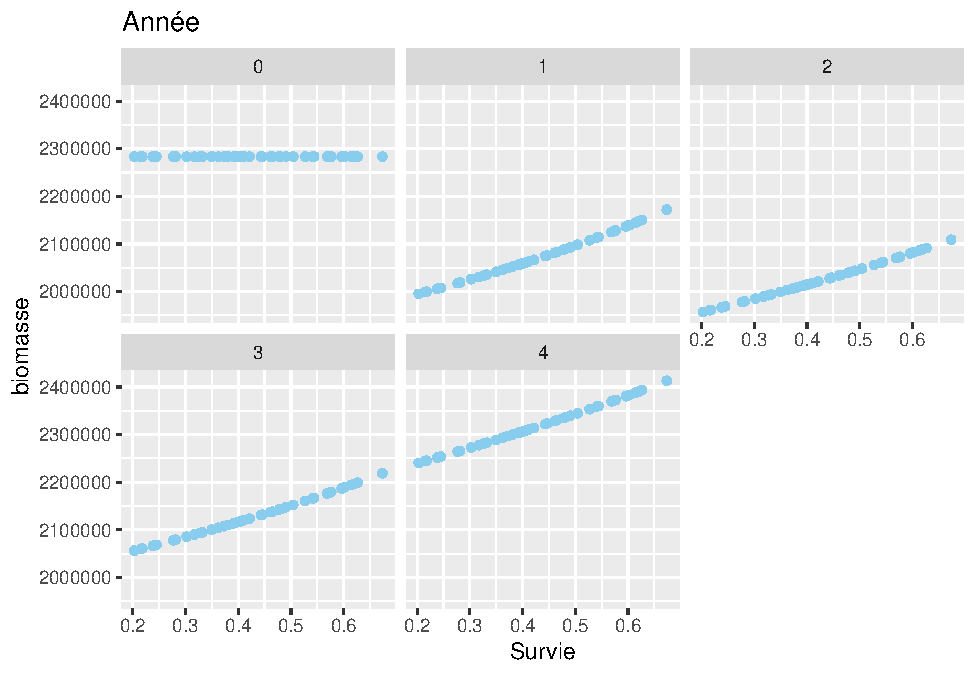
\includegraphics{rapport_files/figure-latex/aocv-1.pdf}

\hypertarget{biomasse-feconde}{%
\subparagraph{Biomasse Feconde}\label{biomasse-feconde}}

La biomasse féconde augmente lorsque la proportion de survie après
relâchement augmente, mais seulement à partir de la deuxième année. Ceci
s'explique car les langoustines relâchées sont celles inférieures à une
certaine taille et par conséquent celles non fécondes. Il faut attendre
un an ou plus pour qu'elle passe à l'âge fécond.

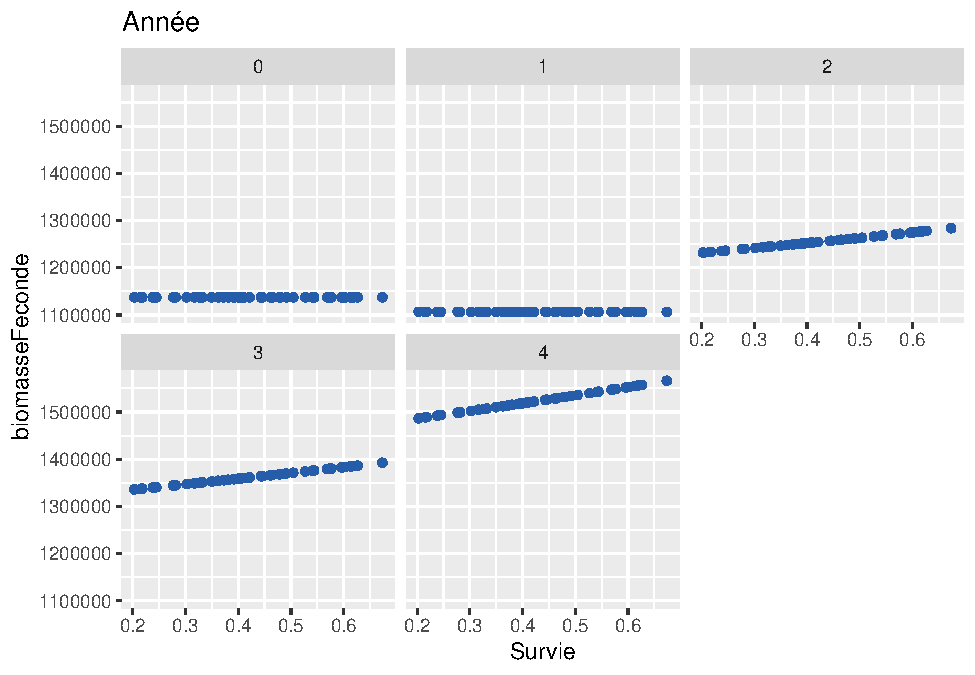
\includegraphics{rapport_files/figure-latex/ccxc-1.pdf}

\hypertarget{poids-des-captures}{%
\subparagraph{Poids des captures}\label{poids-des-captures}}

Le poids des captures de pêche augmente lui aussi lorsque la proportion
de survie après relâchement augmente.

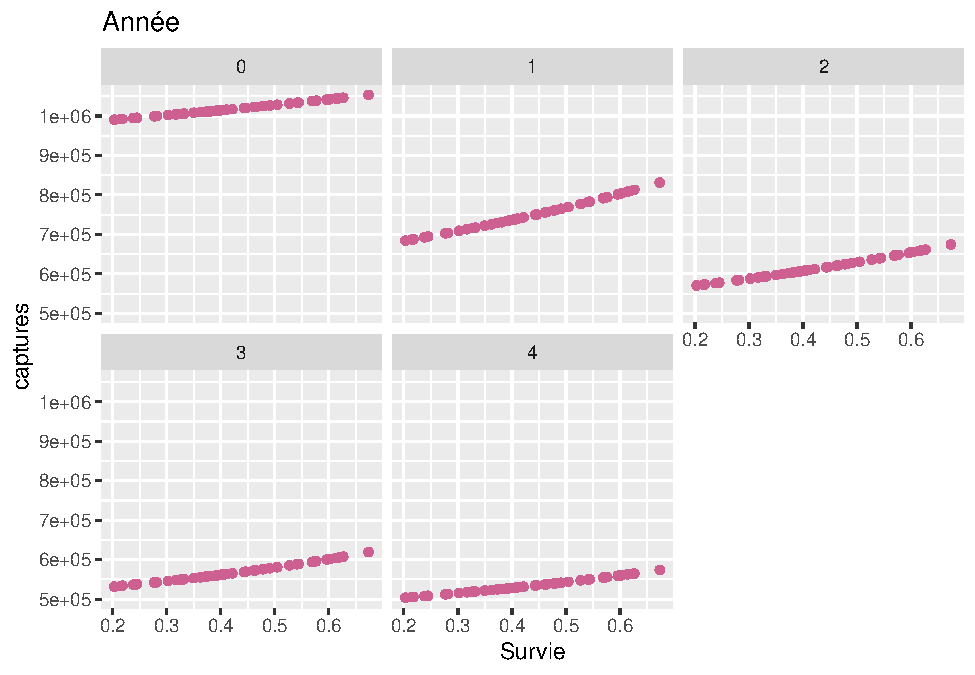
\includegraphics{rapport_files/figure-latex/azsss-1.pdf}

\hypertarget{derive}{%
\paragraph{Derive}\label{derive}}

Etudions les variations des sorties lorsque l'on fait varier la dérive
d'efficacité de pêche.

\hypertarget{biomasse-2}{%
\subparagraph{Biomasse}\label{biomasse-2}}

La diminution de la biomasse suivant l'augmentation de la dérive
s'intensifie au cours des années. Ceci s'explique car si la dérive
augmente cela signifie que les pêcheurs s'améliorent d'années en années.

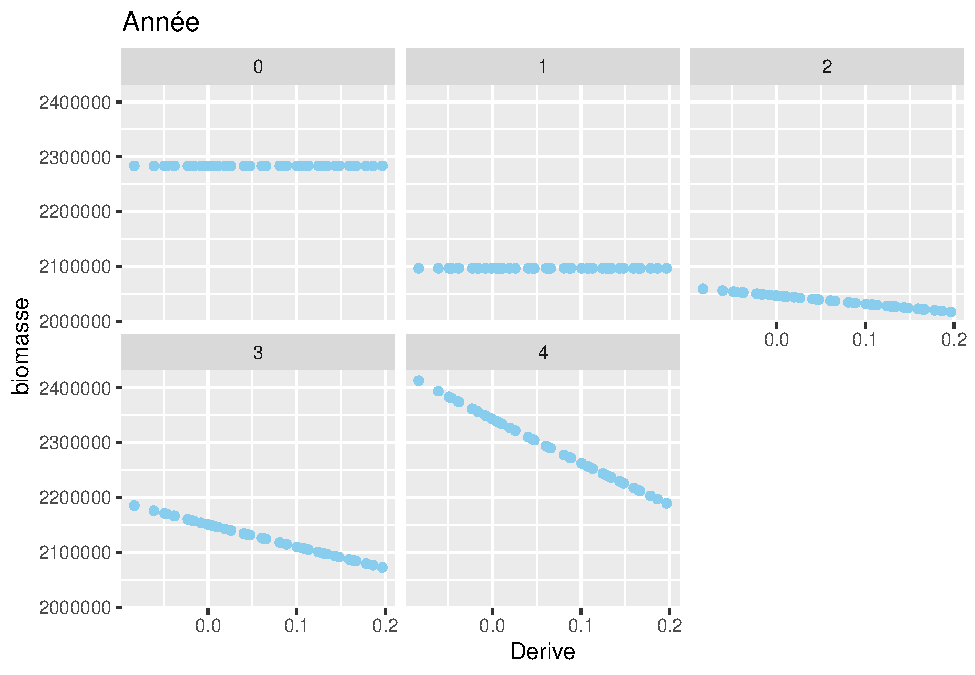
\includegraphics{rapport_files/figure-latex/aos-1.pdf}

\hypertarget{biomasse-feconde-1}{%
\subparagraph{Biomasse Feconde}\label{biomasse-feconde-1}}

La diminution de la biomasse féconde suivant l'augmentation de la dérive
s'intensifie au cours des années. Ceci s'explique car si la dérive
augmente cela signifie que les pêcheurs s'améliorent d'années en années.

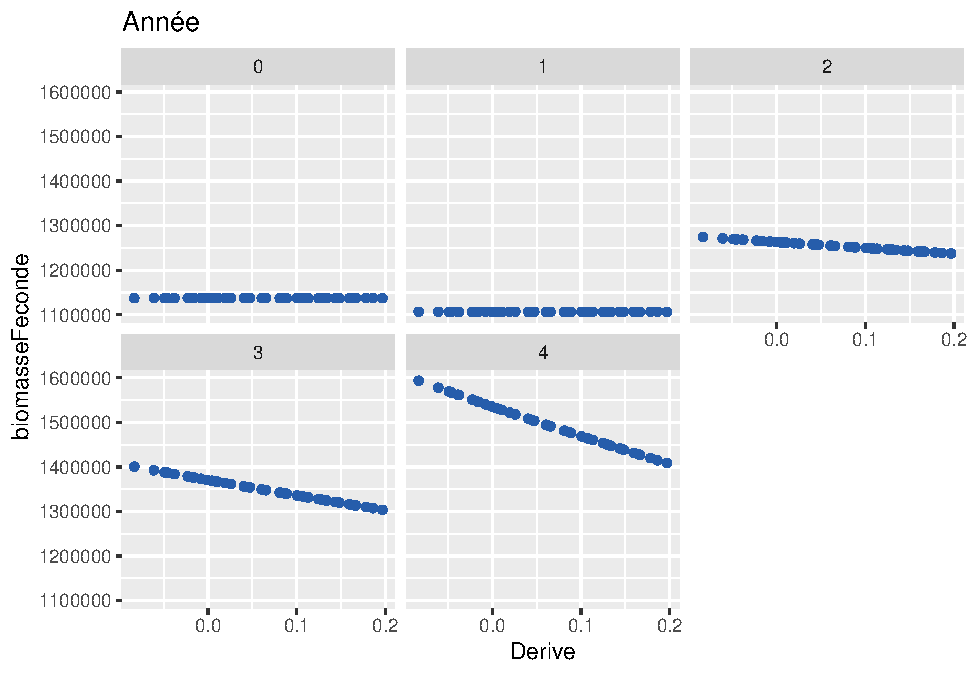
\includegraphics{rapport_files/figure-latex/ccs-1.pdf}

\hypertarget{poids-des-captures-1}{%
\subparagraph{Poids des captures}\label{poids-des-captures-1}}

L'augmentation des captures de pêche suivant l'augmentation de la dérive
s'intensifie au cours des années. Ceci s'explique car si la dérive
augmente cela signifie que les pêcheurs s'améliorent d'années en années.

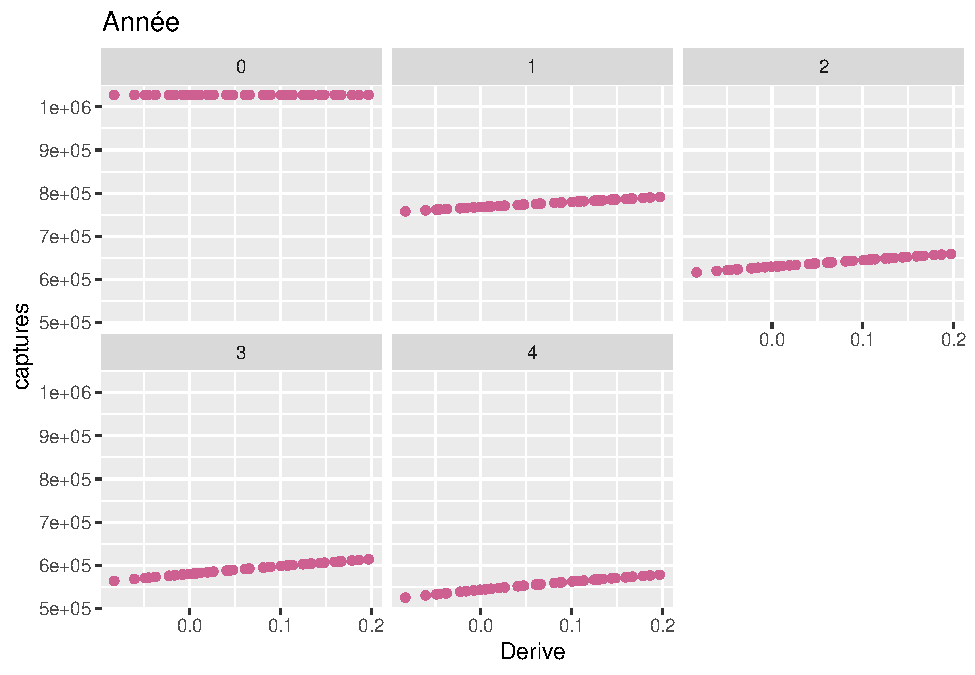
\includegraphics{rapport_files/figure-latex/azs-1.pdf}

\hypertarget{standardisation}{%
\paragraph{Standardisation}\label{standardisation}}

Etudions les variations des sorties lorsque l'on fait varier le facteur
de standardisation des engins.

\hypertarget{biomasse-3}{%
\subparagraph{Biomasse}\label{biomasse-3}}

La biomasse diminue lorsque la standardisation augmente.

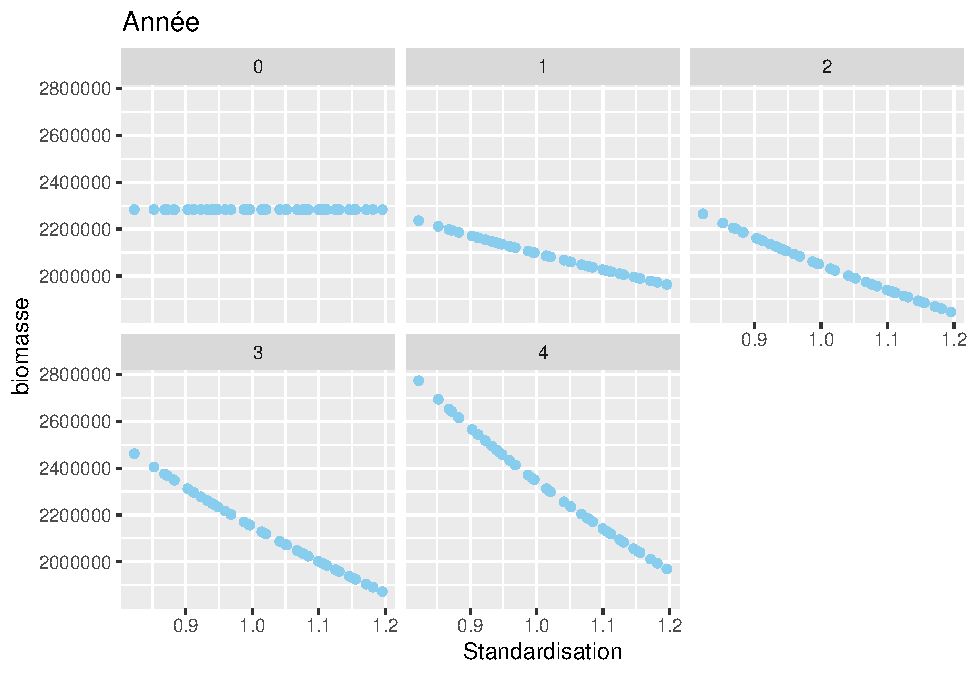
\includegraphics{rapport_files/figure-latex/aps-1.pdf}

\hypertarget{biomasse-feconde-2}{%
\subparagraph{Biomasse Feconde}\label{biomasse-feconde-2}}

La biomasse féconde diminue lorsque la standardisation augmente.

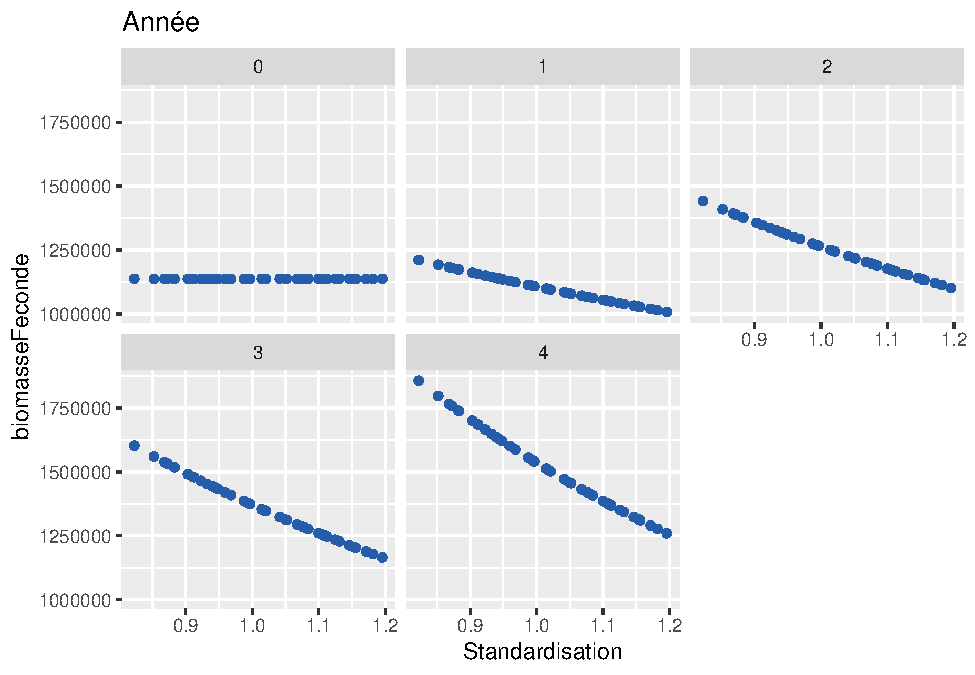
\includegraphics{rapport_files/figure-latex/cp-1.pdf}

\hypertarget{poids-des-captures-2}{%
\subparagraph{Poids des captures}\label{poids-des-captures-2}}

L'année 0, les captures de pêche augmentent lorsque la standardisation
augmente. Les années suivantes, elles stagnent voir diminuent, ce qui
peut s'expliquer par le fait que les pêcheurs en ont trop pêcher l'année
0 et qu'il faut du temps pour que le stock se refasse.

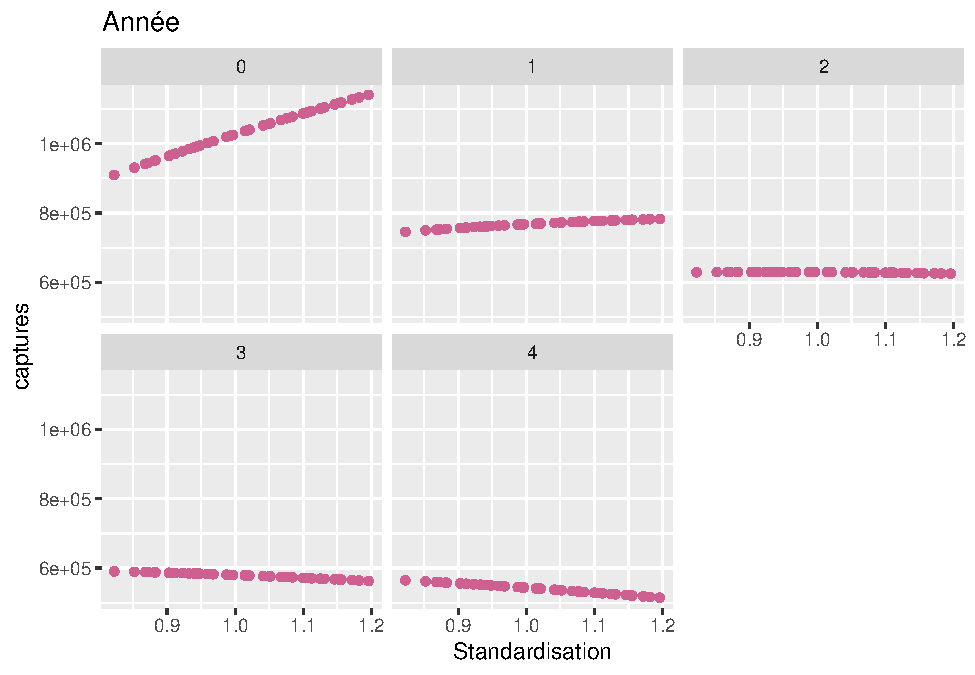
\includegraphics{rapport_files/figure-latex/aq-1.pdf}

\hypertarget{mortalite}{%
\paragraph{Mortalite}\label{mortalite}}

Etudions les variations des sorties lorsque l'on fait varier la
mortalité naturelle.

\hypertarget{biomasse-4}{%
\subparagraph{Biomasse}\label{biomasse-4}}

La biomasse diminue lorsque la mortalité naturelle augmente, le
contraire nous aurait alerté.

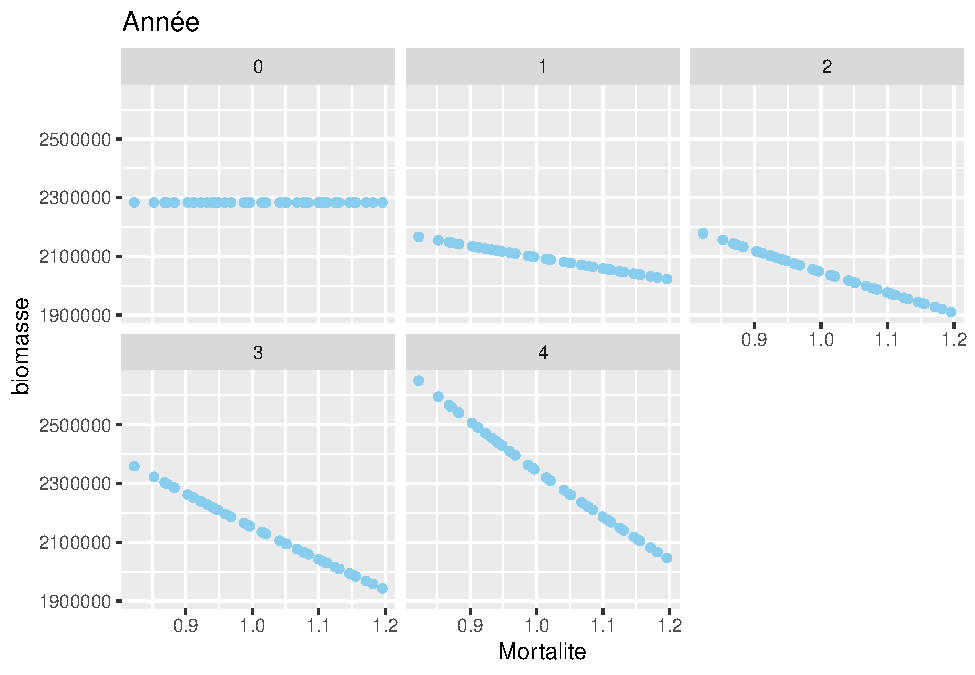
\includegraphics{rapport_files/figure-latex/ag-1.pdf}

\hypertarget{biomasse-feconde-3}{%
\subparagraph{Biomasse Feconde}\label{biomasse-feconde-3}}

La biomasse de géniteurs diminue lorsque la mortalité naturelle
augmente, le contraire nous aurait alerté.

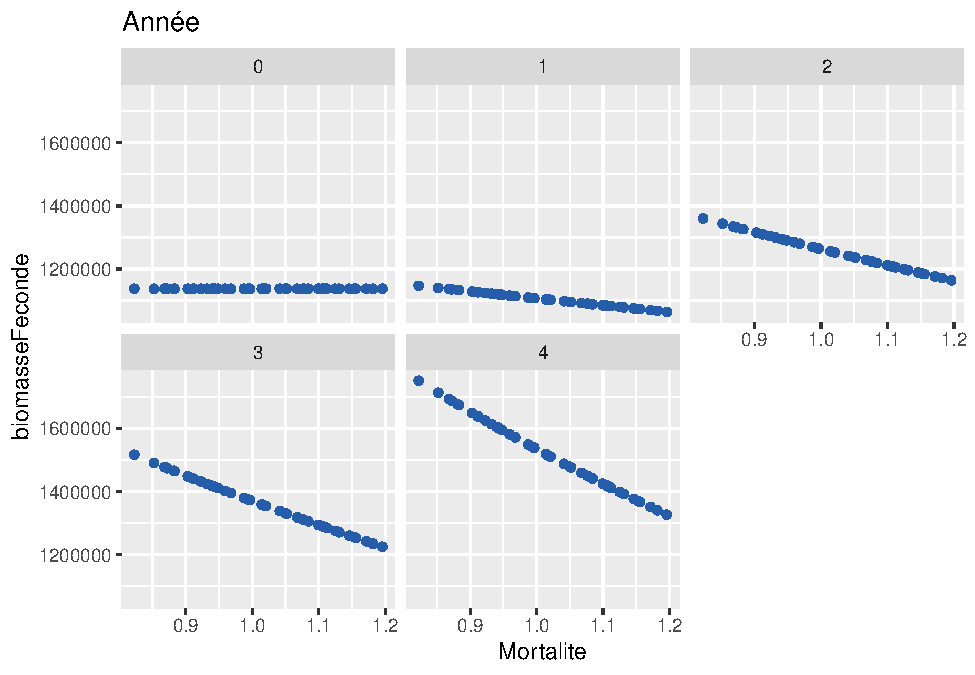
\includegraphics{rapport_files/figure-latex/cm-1.pdf}

\hypertarget{poids-des-captures-3}{%
\subparagraph{Poids des captures}\label{poids-des-captures-3}}

Le poids des captures diminue lorsque la mortalité naturelle augmente,
le contraire nous aurait alerté.

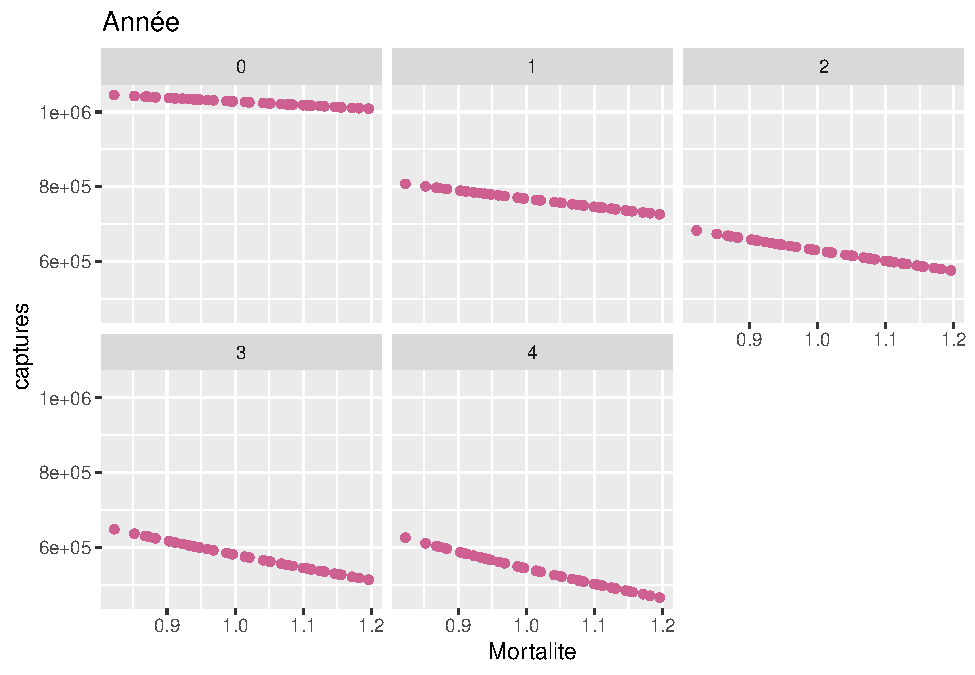
\includegraphics{rapport_files/figure-latex/aj-1.pdf}

\hypertarget{fecondite}{%
\paragraph{Fecondite}\label{fecondite}}

Etudions les variations des sorties lorsque l'on fait varier la
fécondité.

\hypertarget{biomasse-5}{%
\subparagraph{Biomasse}\label{biomasse-5}}

Lorsque la fécondité augmente, l'augmentation de la biomasse
s'intensifie au cours des années. En effet, comme le modèle prédit la
biomasse en unité de masse, les nouveaux nés qui ont un poids faible ne
font pas beaucoup augmenté le poids de la biomasse la 1ère année mais
plus ils grandissent plus ils font augmenté le poids de la biomasse
totale.

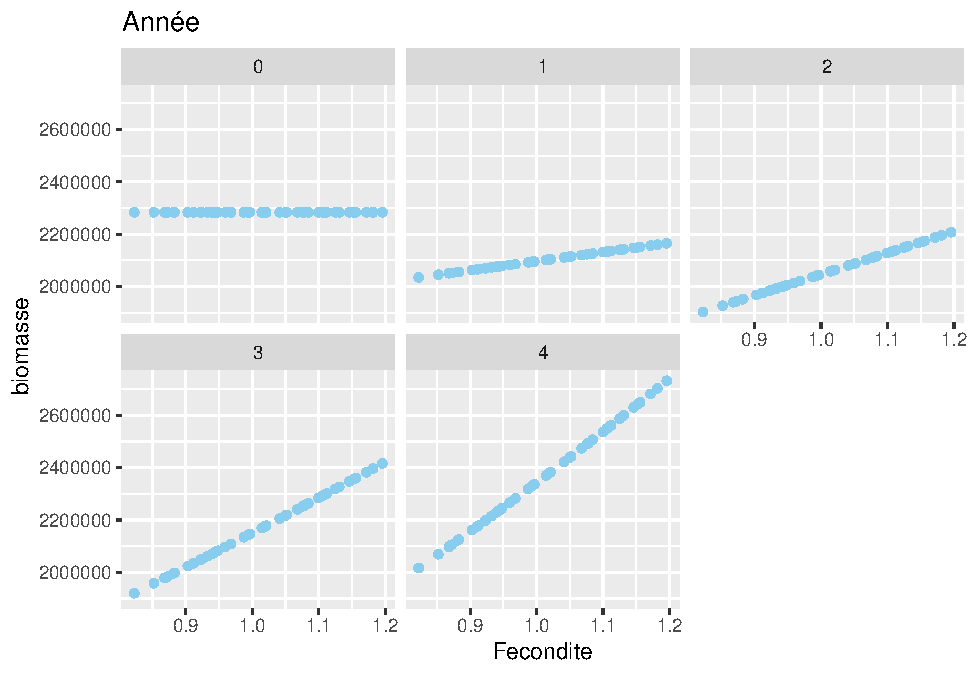
\includegraphics{rapport_files/figure-latex/aocbv-1.pdf}

\hypertarget{biomasse-feconde-4}{%
\subparagraph{Biomasse Feconde}\label{biomasse-feconde-4}}

L'augmentation du taux de fécondité ne fait augmenté la biomasse féconde
qu'à partir de la troisième année car c'est le temps qu'il faut au
nouveaux-nés pour passés de non féconds à féconds.

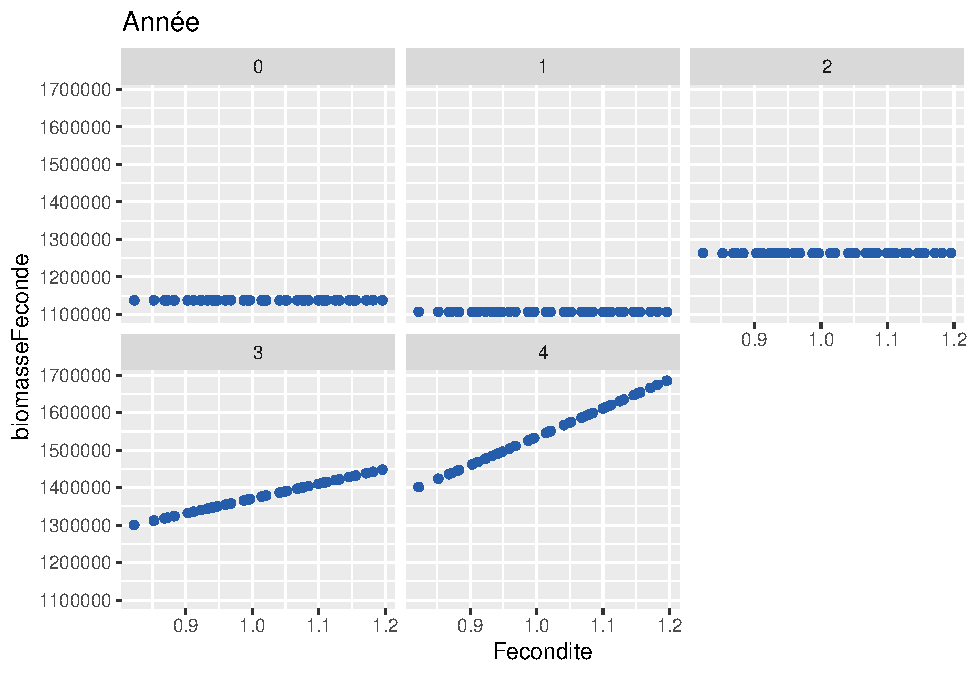
\includegraphics{rapport_files/figure-latex/ccxbc-1.pdf}

\hypertarget{poids-des-captures-4}{%
\subparagraph{Poids des captures}\label{poids-des-captures-4}}

Lorsque la fécondité augmente, l'augmentation du poids des captures
s'intensifie au cours des années car les nouveaux nés grossissent
progressiment.

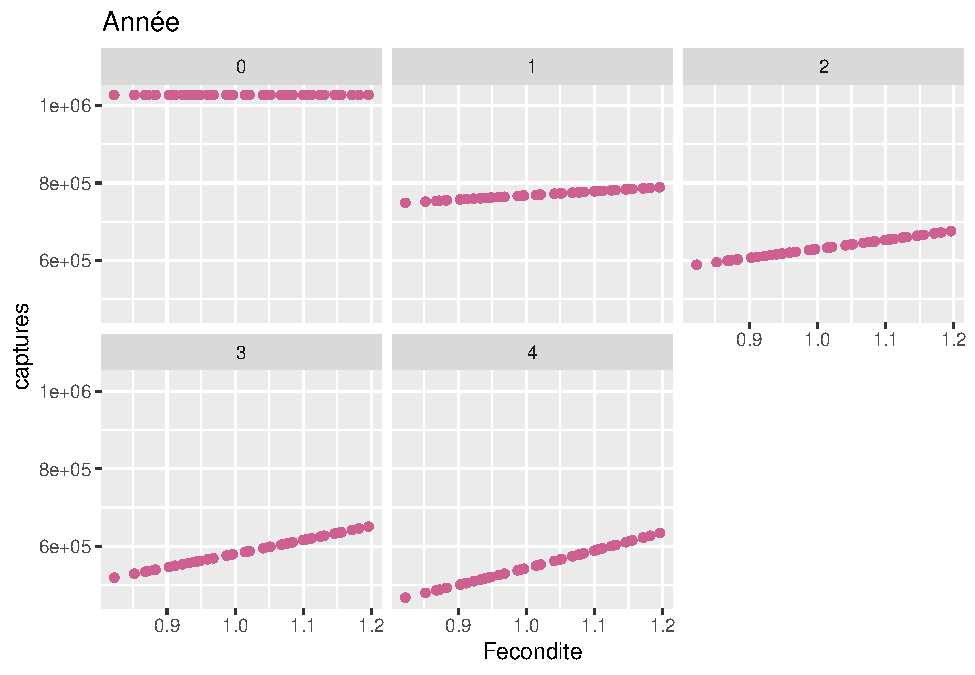
\includegraphics{rapport_files/figure-latex/abzsss-1.pdf}

\hypertarget{quelle-est-la-dynamique-temporelle-des-sorties-et-son-incertitude-lorsque-les-paramuxe8tres-dentruxe9e-varient-conjointement-sur-leur-intervalle-de-confiance-respectif-et-avec-une-hypothuxe8se-de-duxe9pendance}{%
\subsubsection{Quelle est la dynamique temporelle des sorties et son
incertitude lorsque les paramètres d'entrée varient conjointement sur
leur intervalle de confiance respectif et avec une hypothèse de
dépendance
?}\label{quelle-est-la-dynamique-temporelle-des-sorties-et-son-incertitude-lorsque-les-paramuxe8tres-dentruxe9e-varient-conjointement-sur-leur-intervalle-de-confiance-respectif-et-avec-une-hypothuxe8se-de-duxe9pendance}}

\hypertarget{biomasse-6}{%
\paragraph{Biomasse}\label{biomasse-6}}

L'incertitude sur les sorties augmente avec les années. En effet,
l'incertitude se propage à chaque pas de temps.

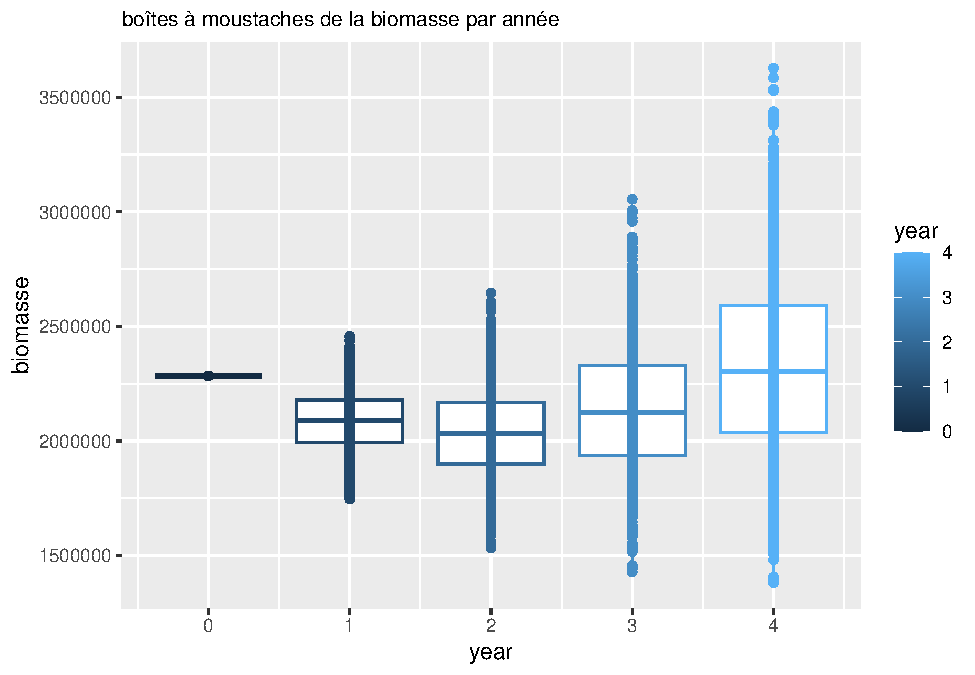
\includegraphics{rapport_files/figure-latex/aus-1.pdf}

\hypertarget{biomasse-feconde-5}{%
\paragraph{Biomasse Feconde}\label{biomasse-feconde-5}}

L'incertitude sur les sorties augmente avec les années. En effet,
l'incertitude se propage à chaque pas de temps.

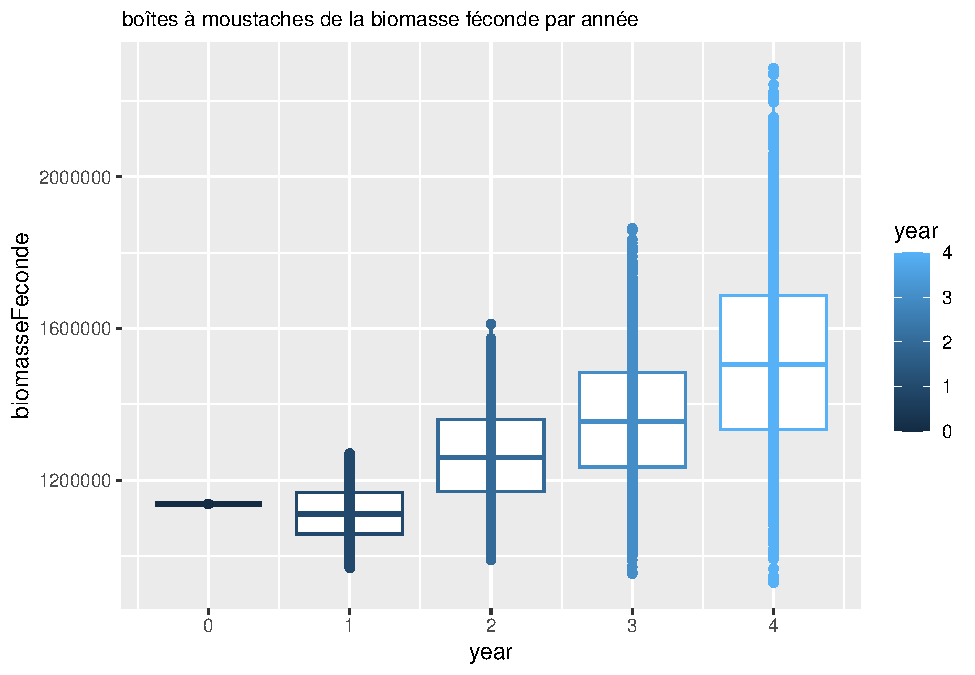
\includegraphics{rapport_files/figure-latex/auxs-1.pdf}

\hypertarget{poids-des-captures-de-puxeache-1}{%
\paragraph{Poids des captures de
pêche}\label{poids-des-captures-de-puxeache-1}}

L'incertitude est très grande la première année, ce qui peut être dû à
la distribution particulière des effectifs initiaux. Ensuite
l'incertitude augmente avec le temps, comme dans les cas précédents.

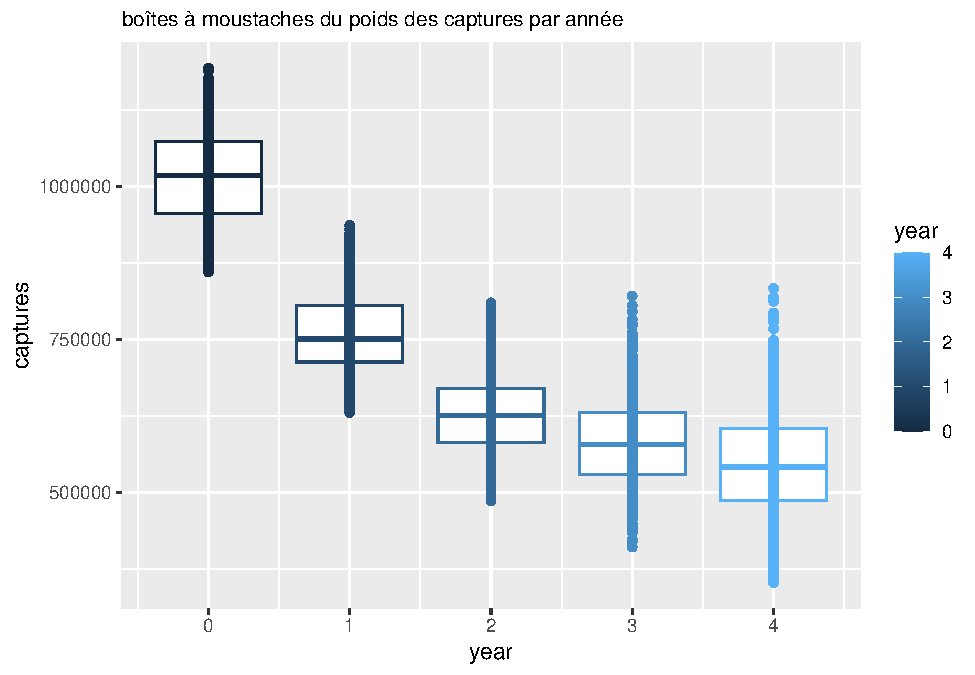
\includegraphics{rapport_files/figure-latex/auxxs-1.pdf}

\hypertarget{analyse-de-sensibilituxe9}{%
\subsection{Analyse de sensibilité}\label{analyse-de-sensibilituxe9}}

\hypertarget{quelle-est-la-dynamique-temporelle-des-indices-de-sobol-mda-lorsque-les-paramuxe8tres-sont-duxe9pendants}{%
\subsubsection{Quelle est la dynamique temporelle des indices de
Sobol-MDA lorsque les paramètres sont dépendants
?}\label{quelle-est-la-dynamique-temporelle-des-indices-de-sobol-mda-lorsque-les-paramuxe8tres-sont-duxe9pendants}}

\hypertarget{biomasse-7}{%
\paragraph{Biomasse}\label{biomasse-7}}

On remarque que pour l'année 1 la standardisation est le paramètre qui
influe le plus sur la biomasse. Viennent ensuite mais loin derrière la
survie, la fécondité et la mortalité. La dérive n'a que très peu
d'importance sur la sortie. Cette ordre va ensuite changé la deuxième
année car la fécondité va devenir plus importante dans le processus de
prédiction tandis que la survie va devenir moins influente. On remarque
que la fécondité devient de plus en plus influente au cours du temps,
jusqu'à devenir 2ème dans le classement des paramètres par ordre
d'influence juste derrière la standardisation. Sa faible influence dans
les premières années s'explique par le fait que le poids des nouveaux
nés ne fait pas beaucoup variés le poids de la biomasse totale en
sortie. Ensuite, comme les nouveaux-nés grandissent la fécondité devient
plus infleuente.

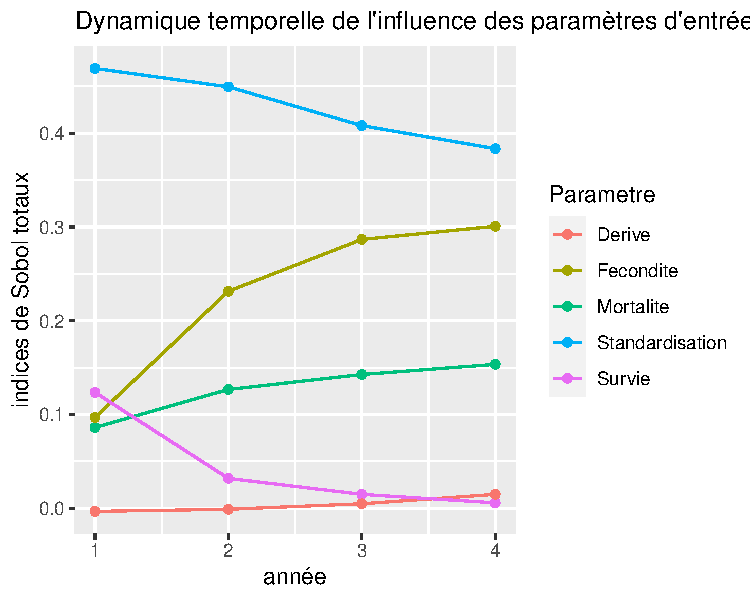
\includegraphics{rapport_files/figure-latex/maptao-1.pdf}

\hypertarget{biomasse-fuxe9conde-1}{%
\paragraph{Biomasse féconde}\label{biomasse-fuxe9conde-1}}

Pour cette sortie, la première année, seulement la standardisation et la
mortalité ont une influence notable. Ensuite l'influence de la fécondité
augmente lentement. En effet, il faut du temps pour que les variations
de la fécondité se reflète sur la biomasse féconde car il faut le temps
que les nouveaux nés deviennent des géniteurs pour être pris en compte
dans cette sortie.

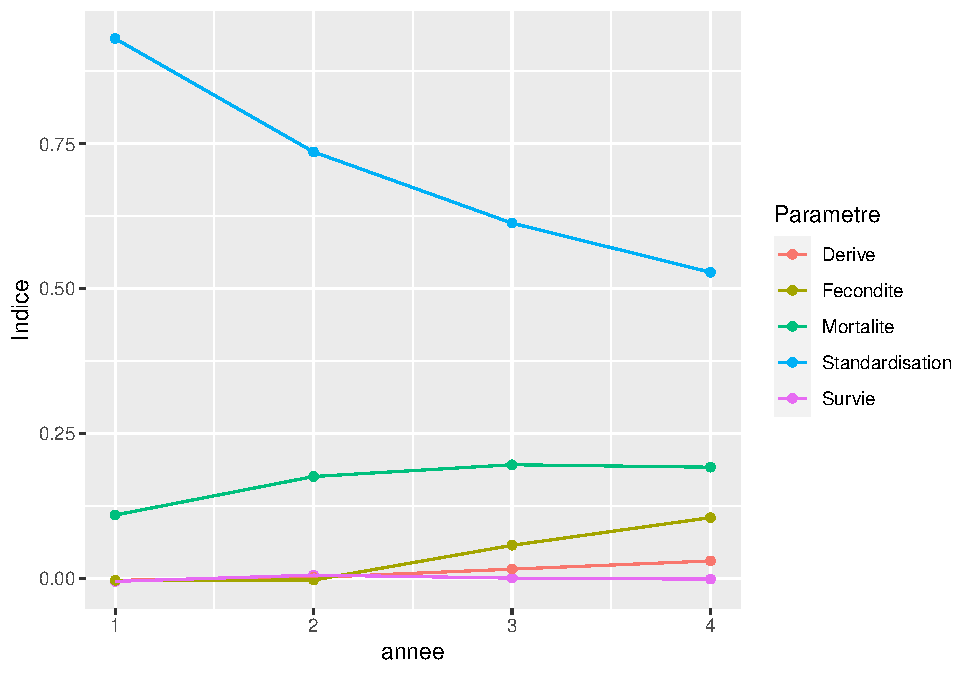
\includegraphics{rapport_files/figure-latex/mapeao-1.pdf}

\hypertarget{poids-des-captures-de-puxeache-2}{%
\paragraph{Poids des captures de
pêche}\label{poids-des-captures-de-puxeache-2}}

La première année, on remarque un classement tout à fait différent pour
cette sortie. La survie est très influente et derrière elle on trouve la
mortalité et la fécondité. Ensuite, comme dans le cas des autres sorties
mais avec d'autres proportions, l'influence de la fécondité et de la
mortalité augmente au cours du temps tandis que celle de la survie
diminue fortement.

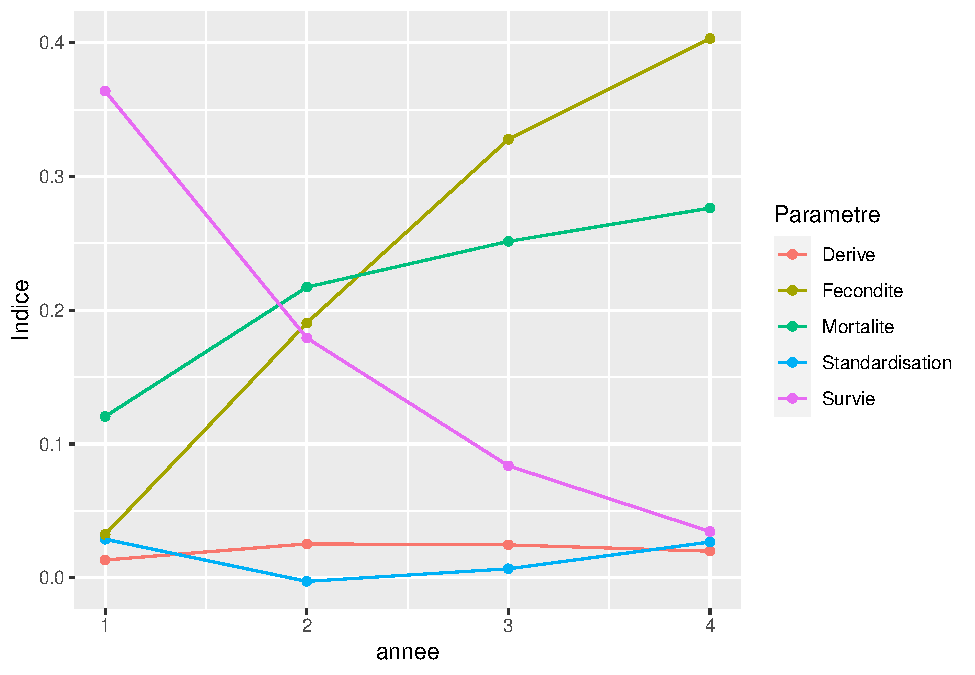
\includegraphics{rapport_files/figure-latex/aoao-1.pdf}

\hypertarget{a-quel-point-nous-serions-nous-trompuxe9s-dans-le-calcul-des-indices-si-nous-navions-pas-mis-de-duxe9pendance-entre-les-paramuxe8tres-dentruxe9e-et-si-nous-avions-utilisuxe9-une-muxe9thode-destimation-ne-prenant-pas-en-compte-la-duxe9pendance}{%
\subsubsection{A quel point nous serions nous trompés dans le calcul des
indices si nous n'avions pas mis de dépendance entre les paramètres
d'entrée ? Et si nous avions utilisé une méthode d'estimation ne prenant
pas en compte la dépendance
?}\label{a-quel-point-nous-serions-nous-trompuxe9s-dans-le-calcul-des-indices-si-nous-navions-pas-mis-de-duxe9pendance-entre-les-paramuxe8tres-dentruxe9e-et-si-nous-avions-utilisuxe9-une-muxe9thode-destimation-ne-prenant-pas-en-compte-la-duxe9pendance}}

Tout d'abord, précisons que, sur les graphiques qui suivent la légende
``estimationIndice'' indique pour quel jeu de données et de quelle
manière les indices ont été calculé. On précise aussi que le calcul des
indices de Sobol-MDA requiert la construction d'un random forest tandis
que le calcul des indices de Sobol totaux se fait directement sur nos
données. Ainsi :

\begin{itemize}
\item
  S-MDA dep signifie que nous avons calculé les indices de Sobol-MDA
  pour des paramètres avec une hypothèse de dépendance (corrélation de
  -0.3 entre survie et dérive et corrélation de -0.5 entre survie et
  mortalité)
\item
  S-MDA indep signifie que nous avons calulé les indices de Sobol-MDA
  pour des paramètres avec une hypothèse d'indépendance.
\item
  ST dep signifie que nous avons calculé les indices de Sobol totaux
  pour des paramètres avec une hypothèse de dépendance.
\item
  ST dep signifie que nous avons calculé les indices de Sobol totaux
  pour des paramètres avec une hypothèse d'indépendance.
\end{itemize}

\hypertarget{biomasse-8}{%
\paragraph{biomasse}\label{biomasse-8}}

Globalement, on remarque que l'hypothèse de dépendance que nous avons
mise ne fait pas varier significativement la valeur des indices, de même
que la méthode de calul utiliser. Néanmoins, on remarque que les indices
qui varient le plus en fonction de l'hypothèse et des méthodes sont ceux
des paramètres sur lesquels on a mis une corrélation. En somme,
l'utilisation d'un méthode classique de calcul des indices de Sobol
totaux et/ou une hypothèse d'indépendance sur les paramètres n'aurait
pas changé les conclusions de notre analyse de sensibilité dans ce cas
précis.

\hypertarget{annee-1}{%
\subparagraph{annee 1}\label{annee-1}}

Pour la mortalité et la survie, on voit des différences notables entre
S-MDA dep et ST Indep. Néanmoins, malgré cette différence, l'indice de
la survie reste plus grand que celui de la mortalité dans les deux cas.

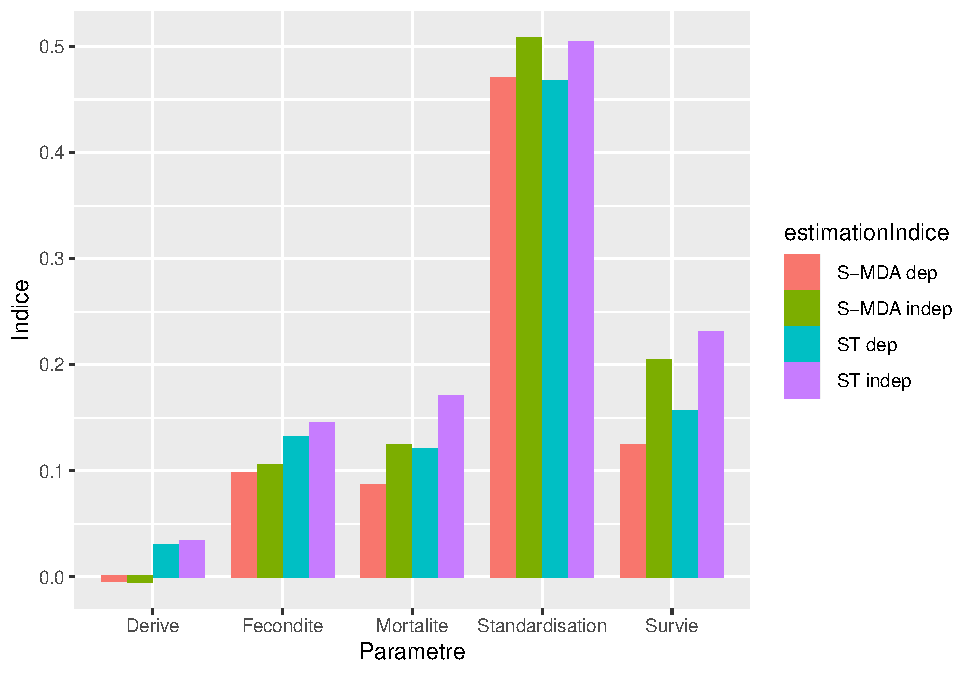
\includegraphics{rapport_files/figure-latex/pfrtygs-1.pdf}

\hypertarget{annee-2}{%
\subparagraph{annee 2}\label{annee-2}}

On note quelques différences notables entre les valeurs mais celles-ci
ne modifient pas le classement des paramètres par ordre d'influence.

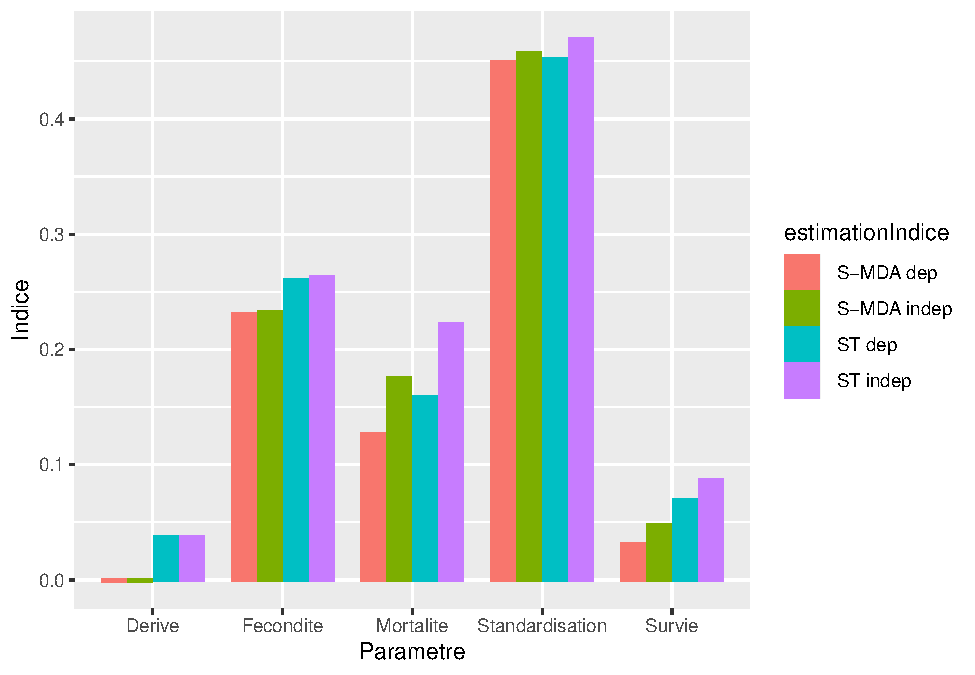
\includegraphics{rapport_files/figure-latex/prtygsrd-1.pdf}

\hypertarget{annuxe9e-3}{%
\subparagraph{année 3}\label{annuxe9e-3}}

Pour les paramètres non-corrélés, les indices sont très rapprochés, ils
sont plus éloignés pour les paramètres corrélés.

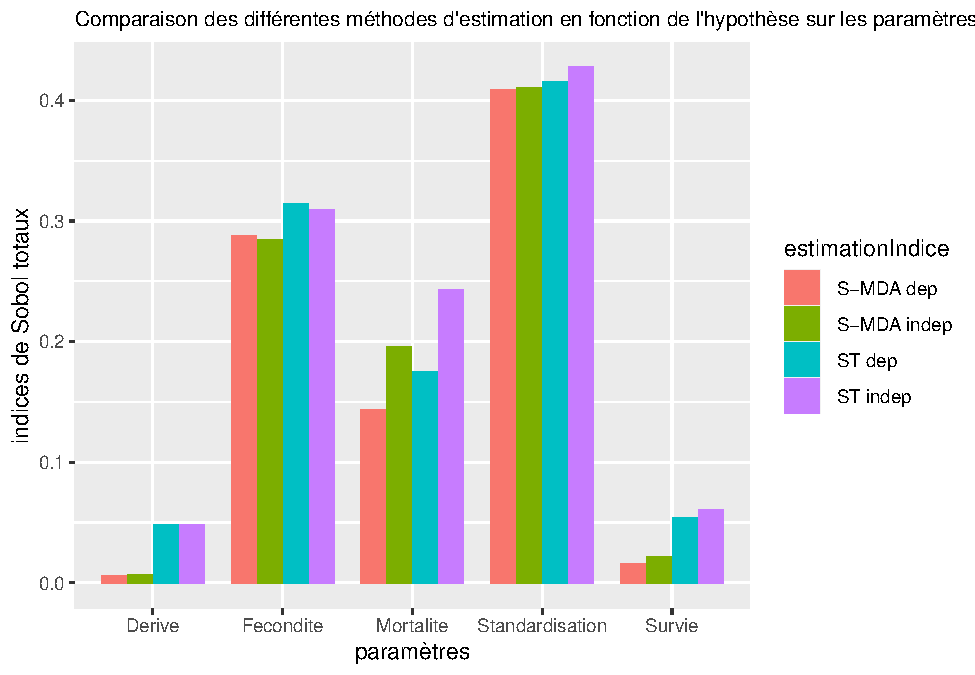
\includegraphics{rapport_files/figure-latex/prtygessf-1.pdf}

\hypertarget{annuxe9e-4}{%
\subparagraph{année 4}\label{annuxe9e-4}}

Pour les paramètres non-corrélés, les indices sont très rapprochés, ils
sont plus éloignés pour les paramètres corrélés.

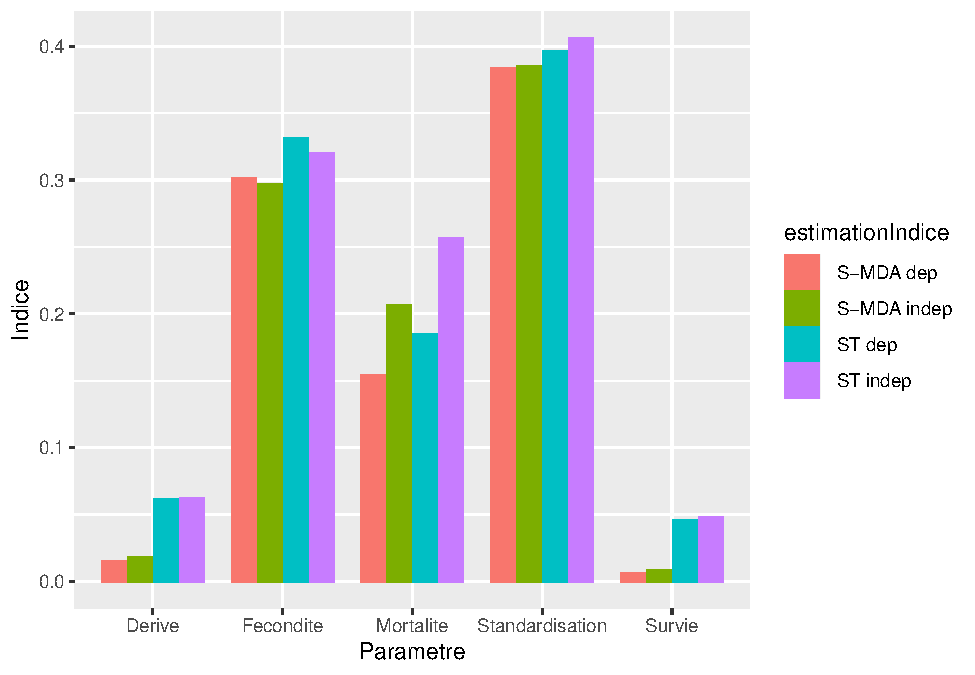
\includegraphics{rapport_files/figure-latex/vhe-1.pdf}

\hypertarget{biomasse-fuxe9conde-2}{%
\paragraph{biomasse féconde}\label{biomasse-fuxe9conde-2}}

Globalement, on remarque que l'hypothèse de dépendance que nous avons
mise ne fait pas varier significativement la valeur des indices, de même
que la méthode de calul utiliser. Néanmoins, on remarque que les indices
qui varient le plus en fonction de l'hypothèse et des méthodes sont ceux
des paramètres sur lesquels on a mis une corrélation. En somme,
l'utilisation d'un méthode classique de calcul des indices de Sobol
totaux et/ou une hypothèse d'indépendance sur les paramètres n'aurait
pas changé les conclusions de notre analyse de sensibilité dans ce cas
précis.

\hypertarget{annee-1-1}{%
\subparagraph{annee 1}\label{annee-1-1}}

On note peu de différences entre les indices, le choix de la méthode et
de l'hypothèse de dépendance ou indépendance n'aurait pas changé les
conclusions de notre analyse de sensibilité.

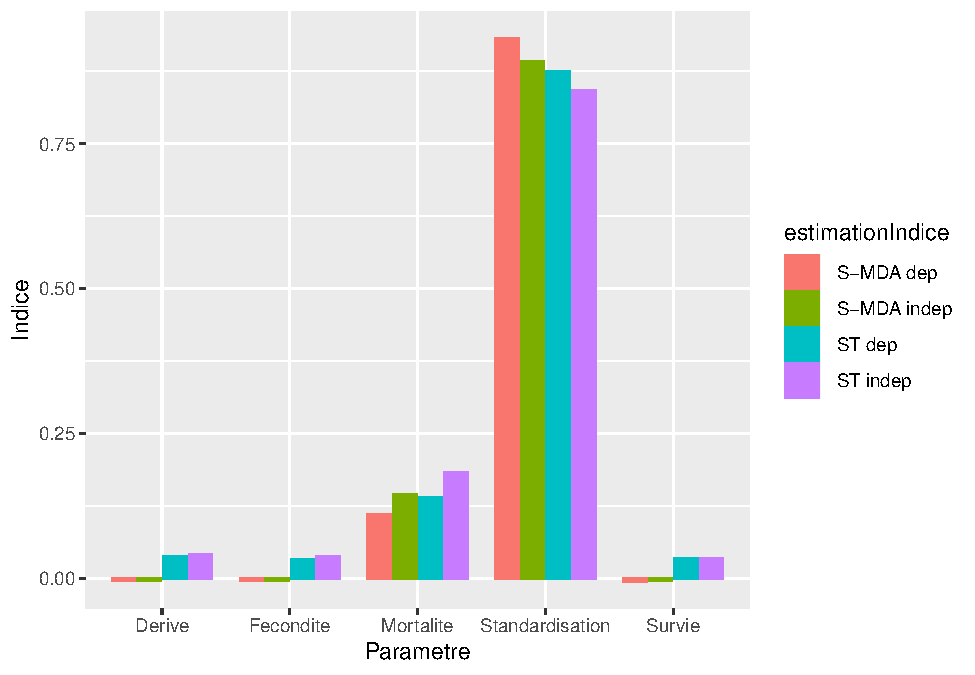
\includegraphics{rapport_files/figure-latex/prteygs-1.pdf}

\hypertarget{annee-2-1}{%
\subparagraph{annee 2}\label{annee-2-1}}

On note peu de différences entre les indices, le choix de la méthode et
de l'hypothèse de dépendance ou indépendance n'aurait pas changé les
conclusions de notre analyse de sensibilité.

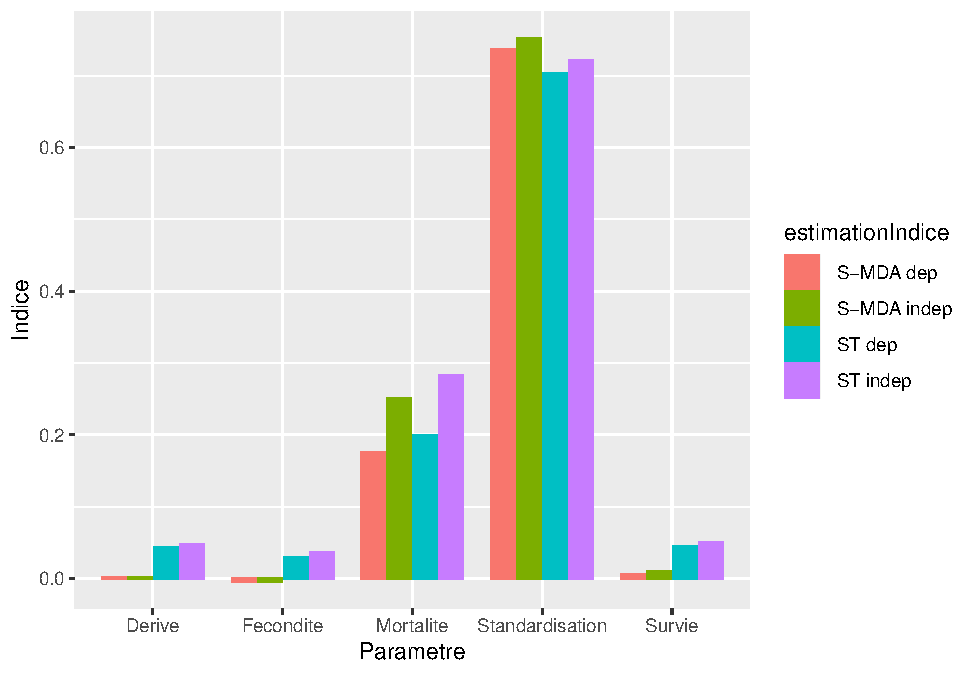
\includegraphics{rapport_files/figure-latex/pertygsd-1.pdf}

\hypertarget{annuxe9e-3-1}{%
\subparagraph{année 3}\label{annuxe9e-3-1}}

On note peu de différences entre les indices, le choix de la méthode et
de l'hypothèse de dépendance ou indépendance, n'aurait pas changé les
conclusions de notre analyse de sensibilité.

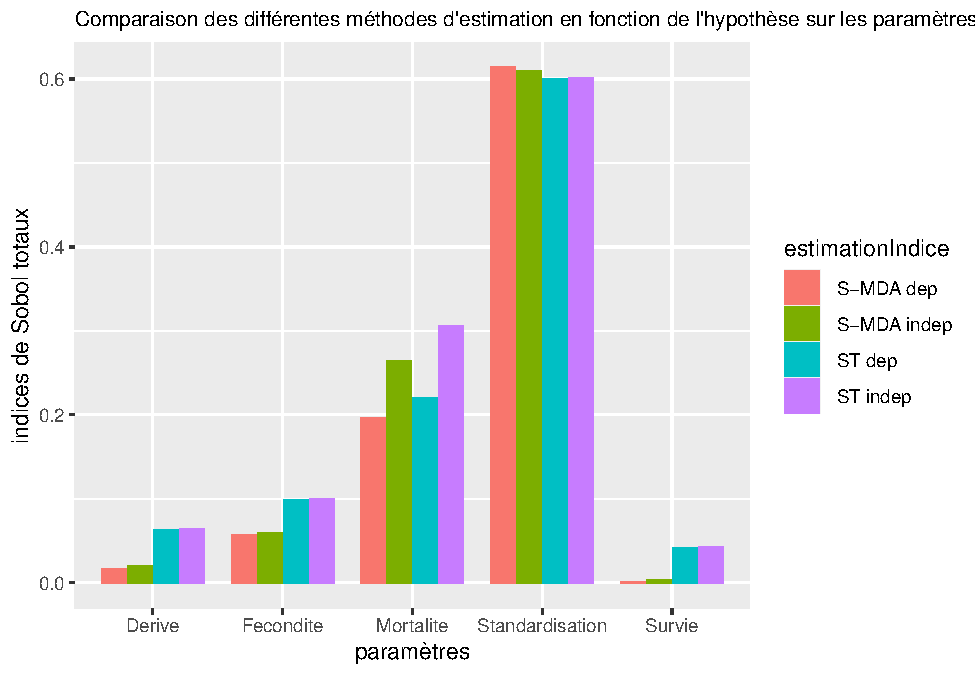
\includegraphics{rapport_files/figure-latex/eprtygssf-1.pdf}

\hypertarget{annuxe9e-4-1}{%
\subparagraph{année 4}\label{annuxe9e-4-1}}

On note peu de différences entre les indices, le choix de la méthode et
de l'hypothèse de dépendance ou indépendance, n'aurait pas changé les
conclusions de notre analyse de sensibilité.

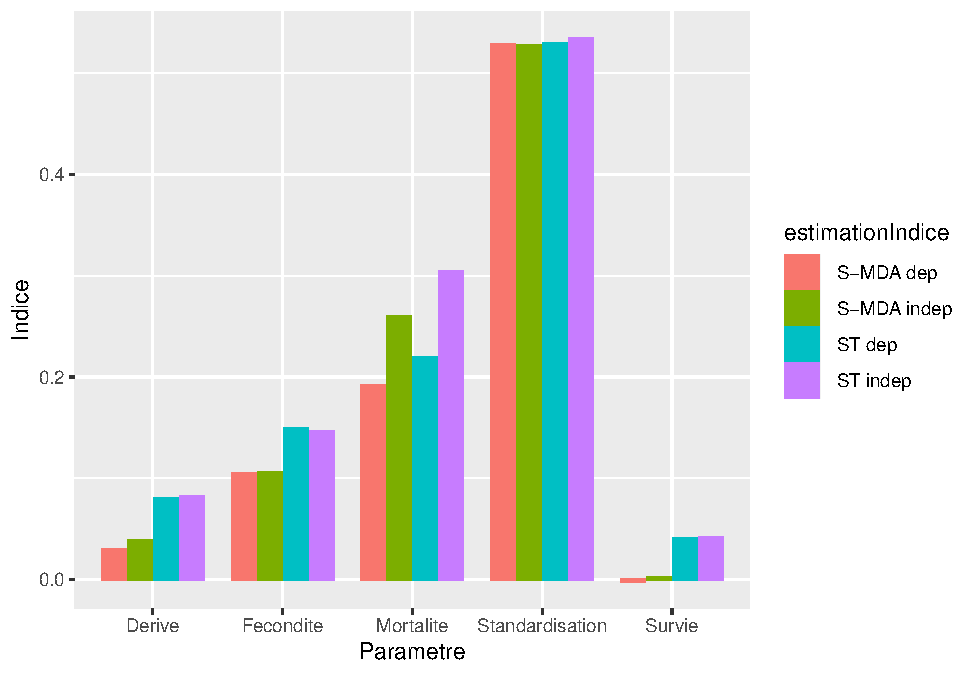
\includegraphics{rapport_files/figure-latex/zvh-1.pdf}

\hypertarget{captures}{%
\paragraph{captures}\label{captures}}

Pour cette sortie, on note davantage de différences entre les indices
que pour les deux autres. En effet, comme les paramètres corrélés survie
et mortalité ont plus d'influence sur cette sortie que sur les autres,
les différences entre les indices selon les méthodes et les hypothèses
sont aussi plus importantes. Néanmoins, ces différences ne changent pas
le classement par ordre d'influence dans la plupart des cas. On remarque
que pour toutes les années, les valeurs des indices ``ST dep'' et
``S-MDA dep'' sont très proches mêmes pour les paramètres corrélés. Cela
signifie que le calcul des indices de Sobol totaux qui n'est normalement
pas adapté aux cas avec dépendance donne de bons résultats dans ce cas
précis.

\hypertarget{annee-1-2}{%
\subparagraph{annee 1}\label{annee-1-2}}

On remarque que quelque soit la méthode de calcul utilisée, pour les
mêmes hypothèses sur les paramètres les indices sont presque identiques.
En revanche, l'hypothèse sur la dépendance (oui ou non) fait varier les
valeurs des indices corrélés.

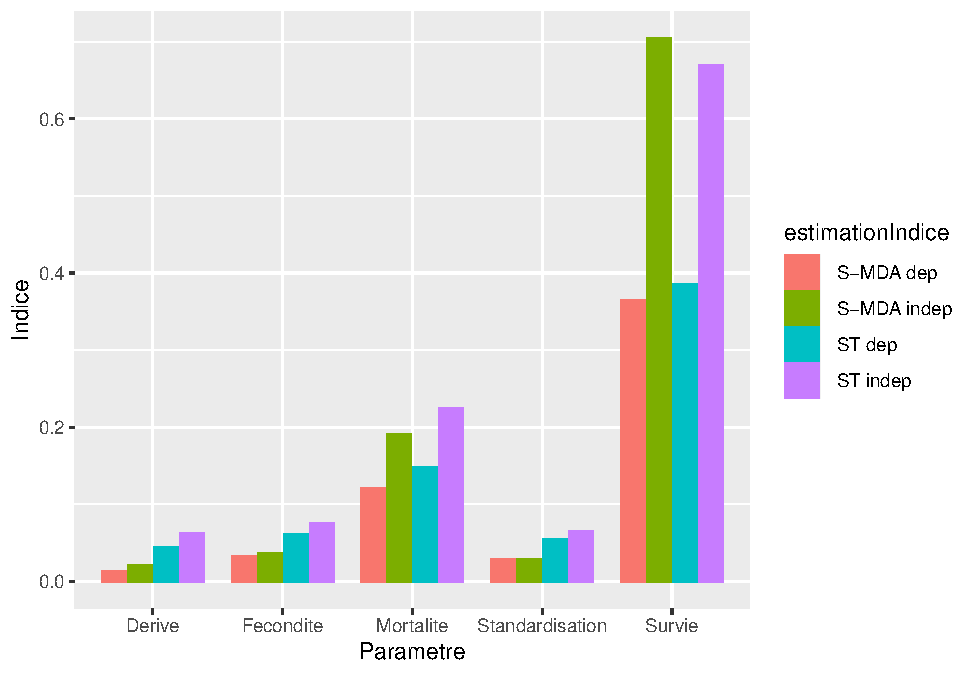
\includegraphics{rapport_files/figure-latex/prtyzgs-1.pdf}

\hypertarget{annee-2-2}{%
\subparagraph{annee 2}\label{annee-2-2}}

On remarque que quelque soit la méthode de calcul utilisée, pour les
mêmes hypothèses sur les paramètres les indices sont presque identiques.
En revanche, l'hypothèse sur la dépendance (oui ou non) fait varier les
valeurs des indices corrélés.

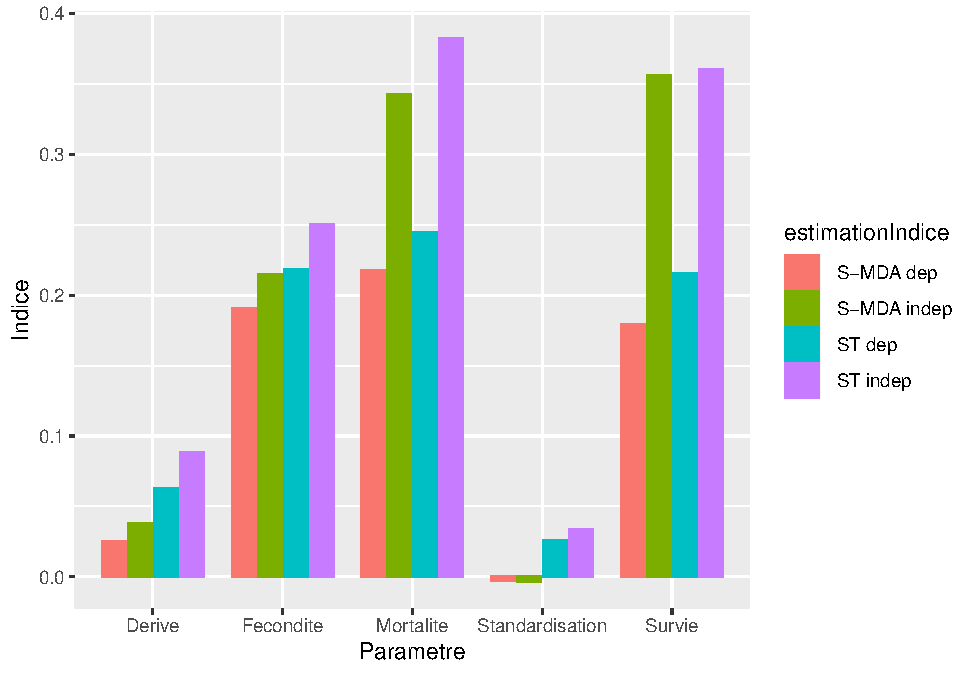
\includegraphics{rapport_files/figure-latex/prtzygs-1.pdf}

\hypertarget{annee-3}{%
\subparagraph{annee 3}\label{annee-3}}

On remarque que quelque soit la méthode de calcul utilisée, pour les
mêmes hypothèses sur les paramètres les indices sont presque identiques.
En revanche, l'hypothèse sur la dépendance (oui ou non) fait varier les
valeurs des indices corrélés.

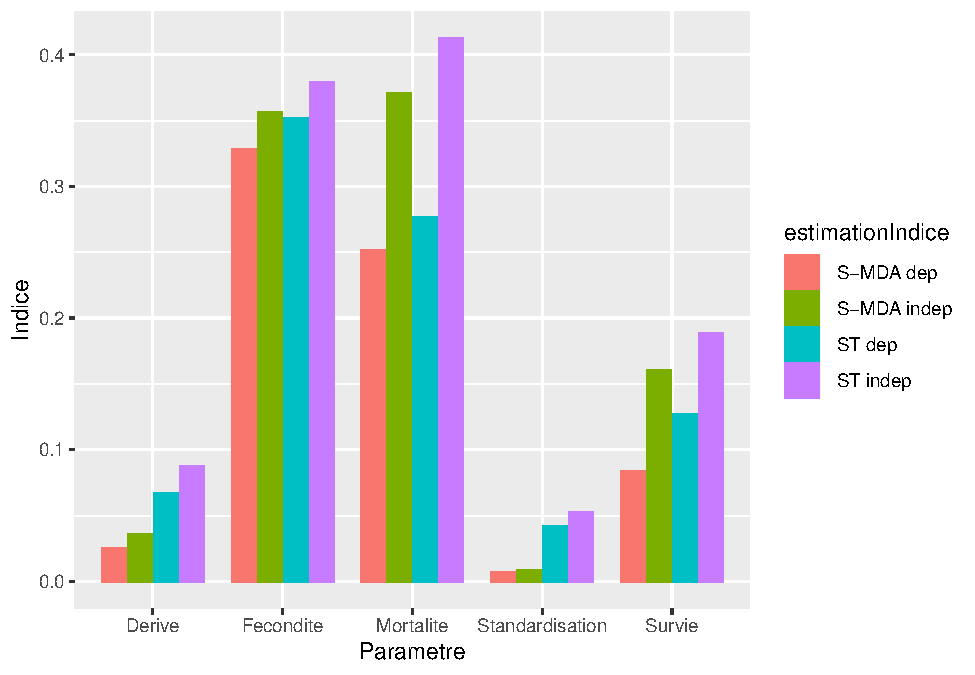
\includegraphics{rapport_files/figure-latex/pzrtygs-1.pdf}

\hypertarget{annee-4}{%
\subparagraph{annee 4}\label{annee-4}}

On remarque que quelque soit la méthode de calcul utilisée, pour les
mêmes hypothèses sur les paramètres les indices sont presque identiques.
En revanche, l'hypothèse sur la dépendance (oui ou non) fait varier les
valeurs des indices corrélés.

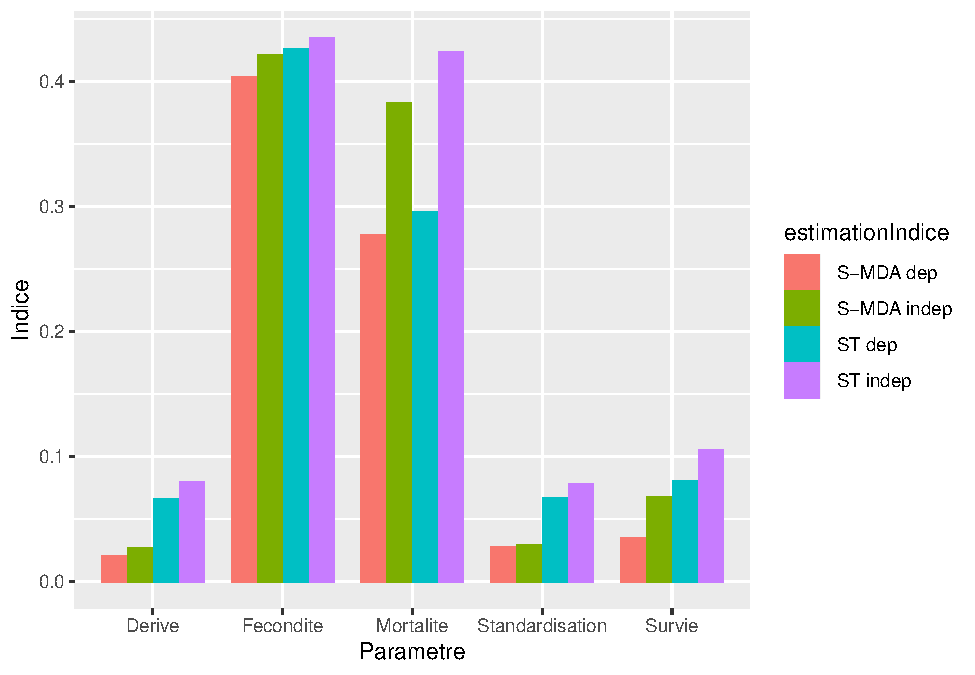
\includegraphics{rapport_files/figure-latex/zprtygs-1.pdf}

\hypertarget{quel-est-leffet-de-la-corruxe9lation-entre-les-paramuxe8tres-dentruxe9e-sur-la-valeur-des-indices-de-sensibilituxe9}{%
\subsubsection{Quel est l'effet de la corrélation entre les paramètres
d'entrée sur la valeur des indices de sensibilité
?}\label{quel-est-leffet-de-la-corruxe9lation-entre-les-paramuxe8tres-dentruxe9e-sur-la-valeur-des-indices-de-sensibilituxe9}}

On remarque que les indices de Sobol-MDA des paramètres corrélés diminue
significativement lorsque la corrélation augmente. Dans certains cas,
l'augmentation de la corrélation entre les paramètres modifie le
classement par ordre d'influence des paramètres.

\hypertarget{biomasse-9}{%
\paragraph{biomasse}\label{biomasse-9}}

\hypertarget{annuxe9e-1}{%
\subparagraph{année 1}\label{annuxe9e-1}}

Les indices des paramètres non corrélés ont tendance à stagner tandis
que ceux de paramètres corrélés diminuent lorsque la corrélation
augmente. Le classement des paramètres change en fonction des valeurs de
corrélation.

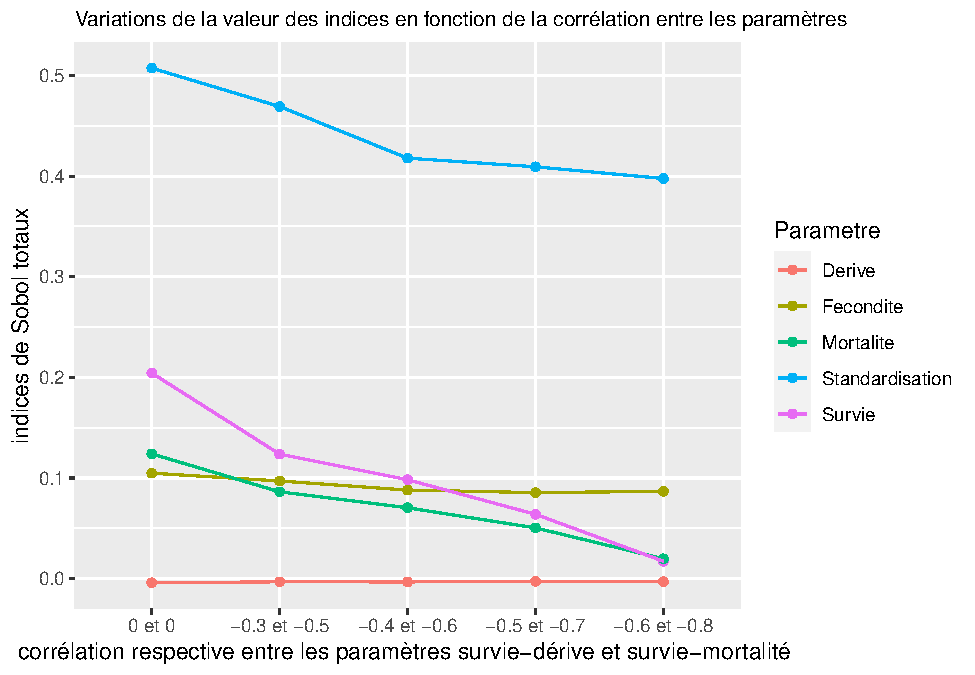
\includegraphics{rapport_files/figure-latex/prztygsbte-1.pdf}

\hypertarget{annee-2-3}{%
\subparagraph{annee 2}\label{annee-2-3}}

Les indices des paramètres non corrélés ont tendance à stagner tandis
que ceux de paramètres corrélés diminuent lorsque la corrélation
augmente. Le classement des paramètres ne change pas en fonction des
valeurs de corrélation.

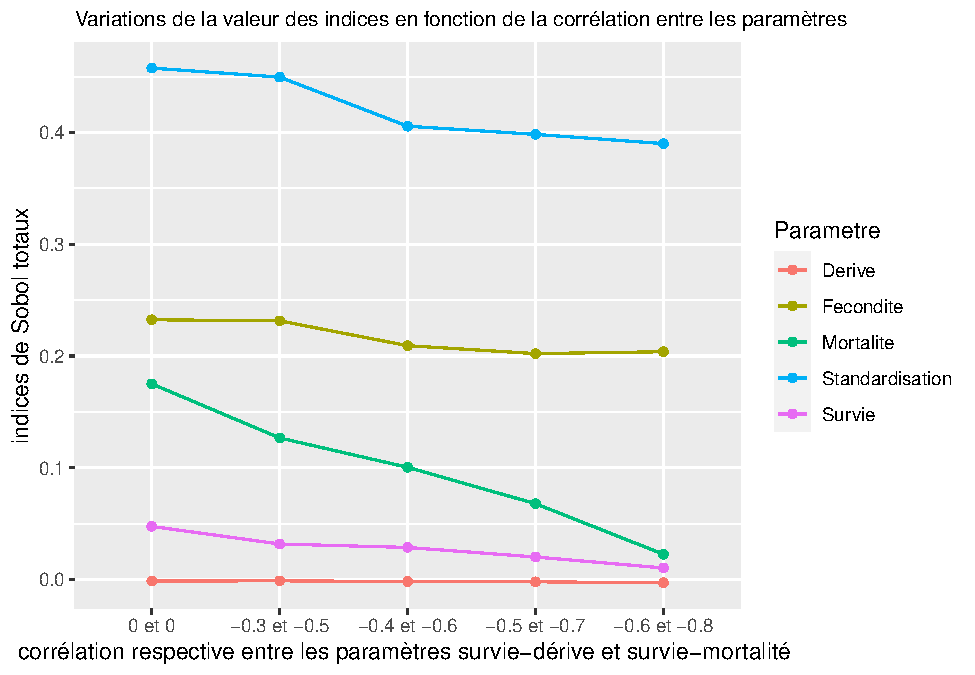
\includegraphics{rapport_files/figure-latex/pzrtygsbte-1.pdf}

\hypertarget{annuxe9e-3-2}{%
\subparagraph{année 3}\label{annuxe9e-3-2}}

Les indices des paramètres non corrélés ont tendance à stagner tandis
que ceux de paramètres corrélés diminuent lorsque la corrélation
augmente. Le classement des paramètres ne change pas en fonction des
valeurs de corrélation.

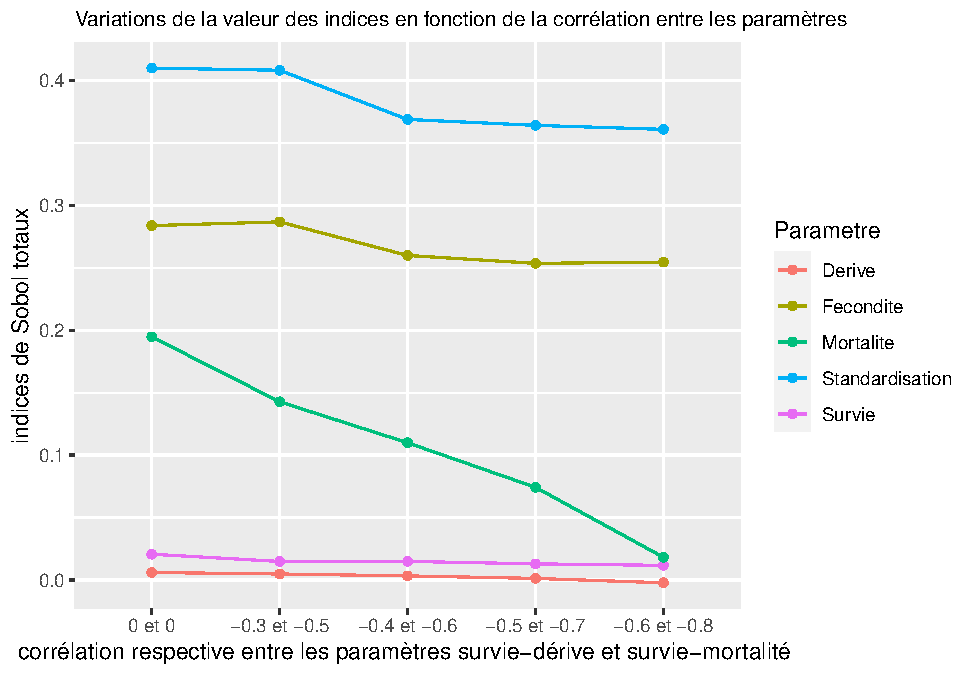
\includegraphics{rapport_files/figure-latex/zprtygsbte-1.pdf}

\hypertarget{annuxe9e-4-2}{%
\subparagraph{année 4}\label{annuxe9e-4-2}}

Les indices des paramètres non corrélés ont tendance à stagner tandis
que ceux de paramètres corrélés diminuent lorsque la corrélation
augmente. Le classement des paramètres change à partir d'une certaines
corrélation.

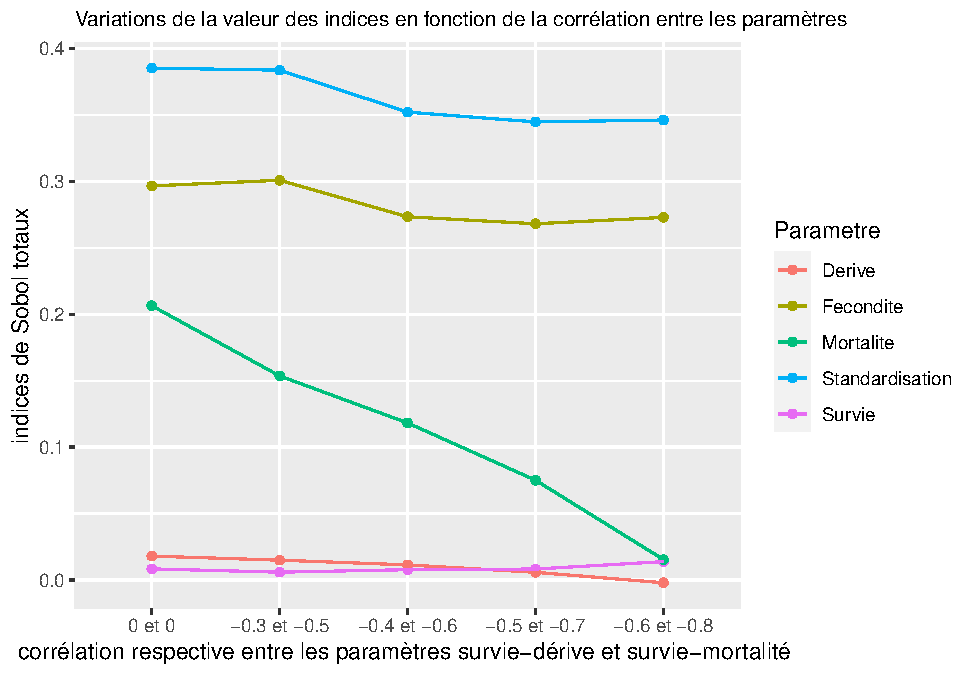
\includegraphics{rapport_files/figure-latex/prtygsbtea-1.pdf}

\hypertarget{biomasse-fuxe9conde-3}{%
\paragraph{biomasse féconde}\label{biomasse-fuxe9conde-3}}

\hypertarget{annuxe9e-1-1}{%
\subparagraph{année 1}\label{annuxe9e-1-1}}

On remarque que l'augmentation de la corrélation fait diminuer l'indice
du paramètre mortalité qui est un paramètre corrélé. On remarque pas
l'effet de l'augmentation de la corrélation car les indices des autres
paramètres corrélés car ils sont très faibles.

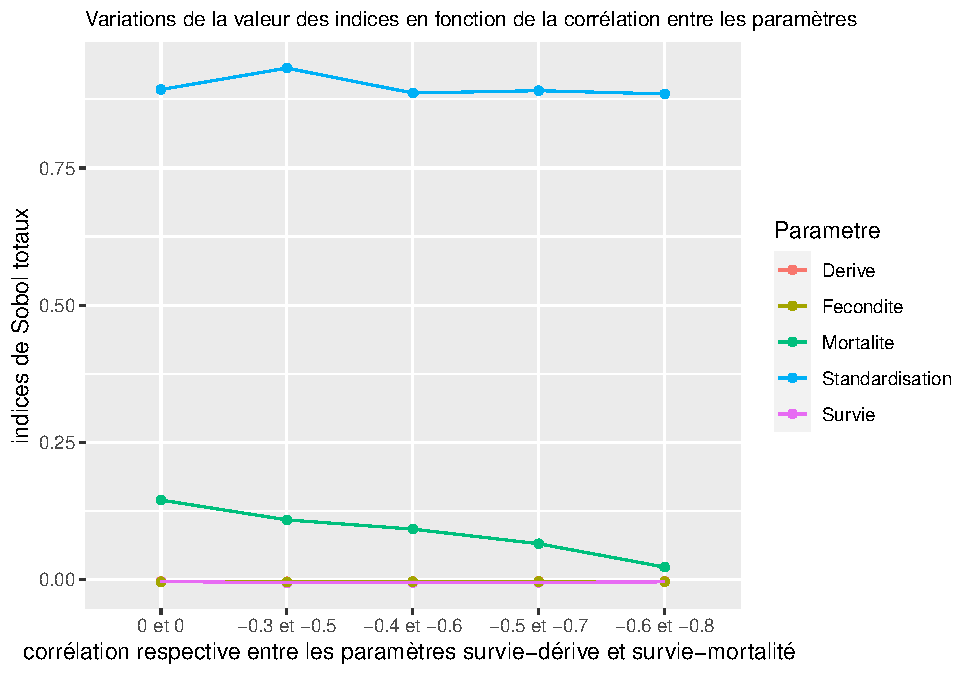
\includegraphics{rapport_files/figure-latex/prtygsbtae-1.pdf}

\hypertarget{annuxe9e-2}{%
\subparagraph{année 2}\label{annuxe9e-2}}

On remarque que l'augmentation de la corrélation fait diminuer l'indice
du paramètre mortalité qui est un paramètre corrélé. On remarque pas
l'effet de l'augmentation de la corrélation car les indices des autres
paramètres corrélés car ils sont très faibles.

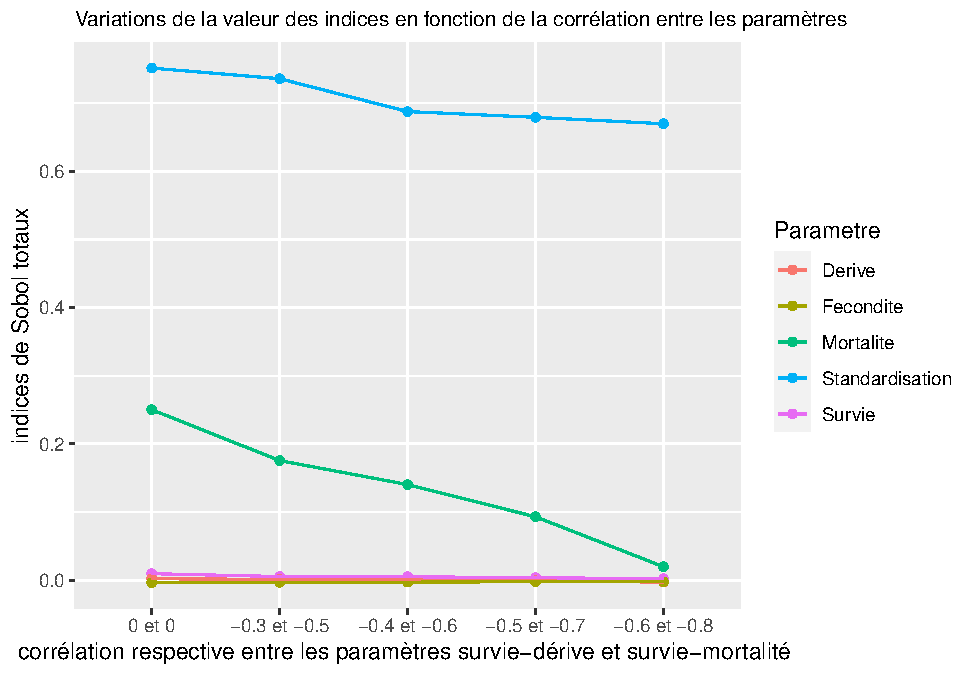
\includegraphics{rapport_files/figure-latex/prtygsbate-1.pdf}

\hypertarget{annuxe9e-3-3}{%
\subparagraph{année 3}\label{annuxe9e-3-3}}

On remarque que l'augmentation de la corrélation fait diminuer l'indice
du paramètre mortalité qui est un paramètre corrélé. On remarque pas
l'effet de l'augmentation de la corrélation car les indices des autres
paramètres corrélés car ils sont très faibles.

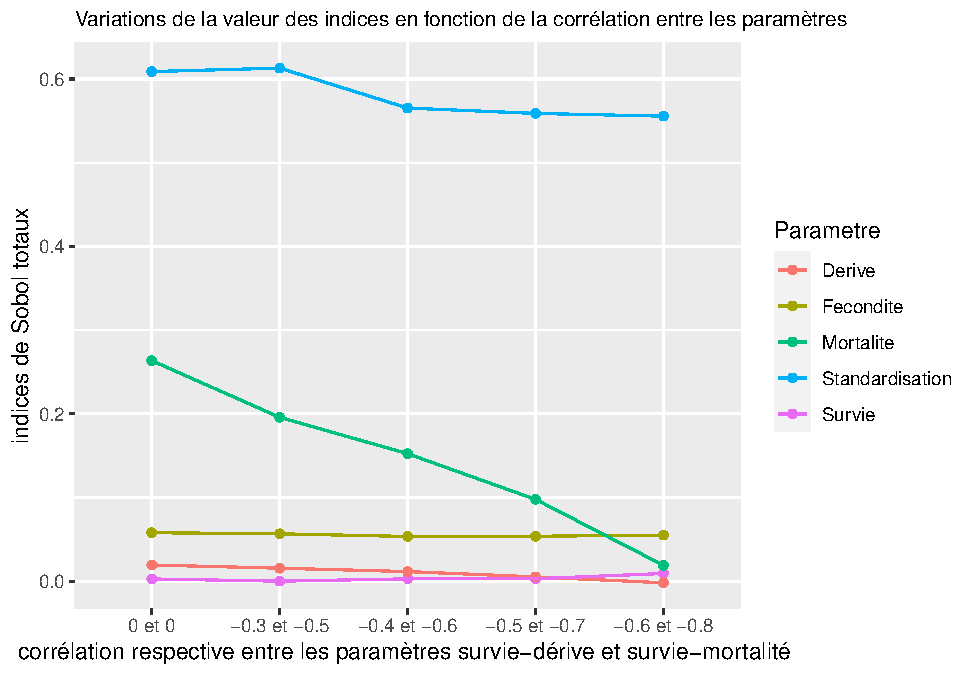
\includegraphics{rapport_files/figure-latex/prtygsabte-1.pdf}

\hypertarget{annuxe9e-4-3}{%
\subparagraph{année 4}\label{annuxe9e-4-3}}

A partir d'une certaine corrélation (-0.5 et -0.7) la mortalité
(paramètre corrélé) dont l'indice diminue fortement devient moins
influente que la fécondité (paramètre non corrélé) dont l'indice a
stagné.

\includegraphics{rapport_files/figure-latex/prtygasbte-1.pdf}

\hypertarget{captures-de-puxeache}{%
\paragraph{captures de pêche}\label{captures-de-puxeache}}

\hypertarget{annuxe9e-1-2}{%
\subparagraph{année 1}\label{annuxe9e-1-2}}

Les paramètres sur lesquels on a mis une corrélation sont très influents
pour corrélation faible ou nulle(surtout la survie). Ainsi la dimintion
de leur importance lorsque la corrélation augmente est flagrante. De
1ère au classement par ordre d'infleunce,la survie est passée avant
dernière avec l'augmentation de la corrélation.

\includegraphics{rapport_files/figure-latex/prtyagsbte-1.pdf}

\hypertarget{annuxe9e-2-1}{%
\subparagraph{année 2}\label{annuxe9e-2-1}}

Les paramètres sur lesquels on a mis une corrélation sont très influents
pour corrélation faible ou nulle (surtout la survie et la mortalité). On
voit leur valeur chuté lorsque la corrélation augmente, ce qui modifie
le classement.

\includegraphics{rapport_files/figure-latex/prtaygsbte-1.pdf}

\hypertarget{annuxe9e-3-4}{%
\subparagraph{année 3}\label{annuxe9e-3-4}}

Les paramètres sur lesquels on a mis une corrélation sont très influents
pour corrélation faible ou nulle (surtout la survie et la mortalité). On
voit leur valeur chuté lorsque la corrélation augmente, ce qui modifie
le classement.

\includegraphics{rapport_files/figure-latex/partygsbte-1.pdf}

\hypertarget{annuxe9e-4-4}{%
\subparagraph{année 4}\label{annuxe9e-4-4}}

Les 2 paramètres influents pour une corrélation nulle sont la survie et
la fécondité. Seul l'influence de la mortalité va diminuer avec
l'augmentation de la corrélation car c'est un paramètre corrélé.

\includegraphics{rapport_files/figure-latex/aprtygsbte-1.pdf}

\hypertarget{conclusion-et-discussion}{%
\section{Conclusion et discussion}\label{conclusion-et-discussion}}

Au cours de cette étude, nous avons pu déterminer le classement des
paramètres par ordre d'influence sur la sortie pour chaque année et pour
chaque sortie du modèle (biomasse, biomasse de géniteurs et captures de
pêche) lorsqu'une hyptothèse de dépendance sur les paramètres a été
mise. Ainsi, cela peut nous mettre d'interpréter le mécanisme de
prédiction du modèle mais aussi de choisir les entrées à fixer pour
diminuer le nombres de paramètres en entrée en perdant le moins possible
en précision. On remarque ensuite que le classement des paramètres
change en fonction de la sortie étudiée. De plus, il évolue en fonction
des années. Pour évaluer l'erreur que l'on aurait pu faire en ne prenant
pas en compte la dépendance entre les paramètres, nous avons aussi
calculé les indices de sensibilité pour des données dont les paramètres
d'entrée sont indépendants. Nous avons remarqué des différences dans les
valeurs des indices, surtout pour les paramètres sur lesquels la
dépendance a été mise. Néanmoins, dans la plupart des cas, cette
différence n'était pas assez grande pour changer le classement par ordre
d'influence des paramètres. On en déduit donc que l'on aurait eu des
résultats assez similaires sans prendre en compte la dépendance.
Finalement, nous avons montré qu'une augmentation de la corrélation
entre les paramètres peut changer le classement par ordre d'influence
des paramètres. La valeur des indices de Sobol MDA des paramètres
corrélés diminue significativement lorsque la corrélation augmente.
Comme le Sobol-MDA mesure l'augmentation de l'erreur du random forest
lorsque l'un des paramètres est retiré du processus de prédiction, il
est normal que l'indice de Sobol total d'un paramètre fortement corrélé
à un autre diminue puisque l'information qu'il apportait est contenue
dans un autre paramètre. Dans une configuration à forte corrélation, il
faut néanmoins rester prudent si l'on souhaite faire du factor fixing
basée sur une sélection des paramètres à faible indice de sensibilité.
En effet, si l'on a 3 paramètres très corrélés par exemple, leurs
indices de sensibilité mesurés avec une méthode prenant en compte la
dépendance sont très petits. On peut alors être tenté de fixer ces 3
paramètres mais on perdra alors beaucoup plus en précision que la somme
des trois indices car il n'en resterait aucun résumant l'information
contenue dans les trois. Pour éviter cela, il faut n'en fixer que deux
et en garder un permettant d'apporter presque autant d'information que
les 3 (grâce à leur corrélation).

Pour approfondir davantage l'étude, nous aurions pu comparer les indices
obtenus à l'aide de la méthode de Sobol-MDA avec les effets de Shapley,
qui prennent également en compte la dépendance, afin d'observer les
différences et de déterminer si le classement reste le même. Par
ailleurs, il aurait été intéressant de calculer les intervalles de
confiance des indices de Sobol-MDA en fonction de l'ajustement du random
forest à notre modèle. Réaliser des simulations sur une période plus
étendue, telle que 10 ans ou 20 ans, aurait également pu être bénéfique,
car les prévisions à long terme du modèle peuvent être utilisée pour
l'aide à prise de décisions. Dans une perspective différente,
l'exploration et l'utilisation des métamodèles obtenus pourraient
également être envisagées.

\hypertarget{annexe}{%
\section{Annexe}\label{annexe}}

\hypertarget{indices-de-sobol}{%
\subsection{Indices de Sobol}\label{indices-de-sobol}}

Les indices de Sobol (Da Veiga et al. (2021)) sont des indices de
sensibilité obtenus grâce à une méthode de décomposition de la variance
fonctionnelle. Il sont compris entre 0 et 1 et leur somme vaut 1. Il
représentent le pourcentage de la variance de la réponse expliquée par
la variable (ou le groupe de variables) pour laquelle ils sont calculés.
Voyons cela plus en détails.

On note dans la suite X le vecteur incluant l'ensemble des variables
d'entrée incertaines : \(X = (X_1 ,...., X_K)\), où K est le nombre de
facteurs incertains. On note finalement G(X) le vecteur des variables de
sortie du modèle associées à X. Si le modèle ne comporte qu'une seule
variable de sortie ou si on ne s'intéresse qu'à une seule des variables
de sortie du modèle, G(X) est un scalaire.

Pour pouvoir écrire la décomposition ANOVA, l'hypothèse 1 suivante doit
être vérifiée.

\begin{itemize}
\tightlist
\item
  \textit{Hypothèse 1} :
\end{itemize}

\textit{Chaque \(X_i\), \(i = 1, . . . , d\), est à valeurs dans un espace mesurable polonais (espace métrique complet et séparable) abstrait \((E_i, B(E_i))\). Ici, \(B(E_i)\) désigne la tribu borrélienne associée à \(E_i\). Pour tout sous-ensemble non vide d'indices \(A \in P_d\) (\(P_d = P([1 : d])\), l'ensemble de tous les sous-ensembles de [1 : d] = {1, . . . , d}), on définit\((E_A, \epsilon_A) = (\Pi_{i\in A} E_i, \otimes_{i\in A} B(E_i))\). On pose \((E,\epsilon)=(E_{[1...d]},\epsilon_{[1...d]})\). Soit \(P_X\) la distribution de probabilité du vecteur aléatoire \(X\). Les composantes \(X_i\) du vecteur aléatoire \(X\) sont supposées être indépendantes ; ainsi, nous avons \(P_X = \prod_{i=1}^{d} P_{X_i}\) avec \(P_{X_i}\) la distribution de probabilité de \(X_i\).}

On pose, pour tout \(A \in P_{d}\) :

\begin{itemize}
  \item \(L^2(P_X) = \{\text{fonctions }f \text{ mesurables sur } (E, \epsilon) : E[f^2(X)] < +\infty\}\)
  \item \(L^2_A = \{f \in L^2(P_X) : f \text{ est mesurable sur }(E_A, \epsilon_A)\}\) 
\end{itemize}

On va maintenant chercher à décomposer des fonctions de \(L^2(P_X)\) sur
des sous-espace de facteurs appropriés.

Soit \(G \in L^2(P_X)\). Sous l'hypothèse 1, il existe une décomposition
unique de \(G\) dans \(L^2(P_X)\) de la forme

\[
G(x) = \sum_{A \in P_d} G_A(x_A)
\]

telle que les deux propriétés suivantes soient satisfaites :

\begin{enumerate}
\def\labelenumi{\arabic{enumi}.}
\tightlist
\item
  \(G_\emptyset\) est constant.
\item
  \(\forall A \in P_d, A \neq \emptyset, \forall i \in A, \int_{E_i} G_A(x_A) \, P_{X_i}(dx_i) = 0\)
\end{enumerate}

La solution unique s'exprime, \(\forall A \in P_{d},\)

\[
G_A(x_A) = \sum_{B \subseteq A} (-1)^{|A| - |B|} \mathbb{E}[G(X) \,|\, X_B = x_B]
\]

Pour tout \(A \in P_d, A \neq \emptyset\), posons
\(V_A = \text{Var } G_A(X_A)\). Alors, sous l'hypothèse 1, nous obtenons
\[
V = \text{Var } G(X) = \sum_{A \in P_d, A \neq \emptyset} V_A.
\] De plus, pour tout \(A \in P_d, A \neq \emptyset\), on : \[
V_A = \sum_{B \subset A} (-1)^{|A| - |B|} \text{Var } \mathbb{E}[G(X)|X_B]
\] On peut démontrer que \(G_A\) est la meilleure approximation de \(G\)
dans le sens de \(L^2(P_X)\), appartenant à \(L^2_A\) et étant
orthogonal (par rapport au produit scalaire hilbertien dans
\(L^2(P_X)\)) à toute fonction dans \(L^2_{A_0}, A_0 \subsetneq A\).

Maintenant que nous avons défini le cadre théorique sur lequel repose la
définition des indices de Sobol, voyons leur expression mathématique.

Soit \(G \in L^2(P_X)\) et on suppose que l'hypothèse 1 est satisfaite.
Soit \(A \in P_d\).

\begin{itemize}
\item
  L'indice de Sobol associé à A est défini tel que : \[
  S_A = \frac{V_A}{V} = \frac{\sum_{B \subseteq A} (-1)^{|A| - |B|} \text{Var} \left[E[G(X) | X_B]\right]}{\text{Var} [G(X)]}.
  \]
\item
  \(S_j\) est l'indice de Sobol associé au singleton \(\{j\}\). On
  l'appelle l'indice d'ordre un pour la variable d'entrée \(X_j\). Plus
  généralement, si \(p = |A|\), alors \(S_A\) est appelé l'indice de
  Sobol d'ordre p associé à \(X_A\).
\item
  L'indice de Sobol fermé associé à l'ensemble A est défini tel que
  \[ S^{\text{clos}}_A = \sum_{A'\subset A}S_{A'}=\frac{\text{Var} E[G(X)|X_A]}{\text{Var} G(X)} \]
  Cet indice est également appelé l'indice de Sobol du premier ordre
  associé au vecteur d'entrée \(X_A\).
\item
  L'indice de Sobol total associé à \(X_A\) est défini tel que : \[
  S^{T}_A = 1 - S^{\text{clos}}_{A^c}.
  \]
\end{itemize}

Les indices de Sobol possèdent les propriétés suivantes :

Soit \(G \in L^2(P_X)\). Supposons que l'hypothèse \(1\) est satisfaite.
Nous avons :

\begin{enumerate}
\def\labelenumi{\arabic{enumi}.}
\item
  \[
  \sum_{A \in P_d} S_A = 1.
  \]
\item
  Si \(\sum_{j=1}^d S_j = 1\), alors le modèle est additif (c'est-à-dire
  que \(G\) est simplement la somme de fonctions impliquant seulement
  une variable).
\item
  \[
  S_{A}^T = \frac{E [ Var (G(X)|X_{\bar{A}}) ]}{Var G(X)} =\sum_{A' \in P^d, A' \cap A \neq \emptyset} S_{A'}\tag{3}
  \]
\end{enumerate}

Pour \(A = \{j\}\), la dernière égalité devient
\(S_j = \sum_{A' \in P^d, j \in A'} S_{A'}\).

Remarque : La première égalité dans l'équation (3) est toujours vraie
même pour les composantes dépendantes de \(X\). Ce n'est plus le cas
pour la deuxième.

\hypertarget{effets-de-shapley}{%
\subsection{Effets de Shapley}\label{effets-de-shapley}}

\hypertarget{contexte-et-pruxe9requis}{%
\subsubsection{Contexte et prérequis}\label{contexte-et-pruxe9requis}}

Les effets de Shapley permettent d'attribuer la valeur créée par une
équipe à ses membres (Zaccour et al. (1988)). Appliqués à l'analyse de
sensibilité, on peut considérer que les variables d'entrée
\((X_1, ..., X_d)\) représentent les membres de l'équipe et que la
valeur de la sortie Y=G(X) représente la valeur créée par l'équipe. On
suppose que \(G(X) \in L^2(P_X)\) où \(P_X\) est la loi de probabilité
de X. Les effets de Shapley résultent d'une allocation directe d'une
part de la variance de la sortie à chaque entrée(Da Veiga et al.
(2021)). Voyons cela plus en détails.

Considérons une fonction charactéristique val définie sur \(P_d\)
(\(P_d = P([1 : d])\), l'ensemble de tous les sous-ensembles de {[}1 :
d{]} = \{1, . . . , d\}) et à valeurs dans \(\mathbb{R}_+\) telle que
\(val(\emptyset)=0\). Basée sur cette fonction charactéristique, une
valeur \(\Phi_j\) est attribuée à chaque variable d'entrée \(X_j\) (à
chaque joueur dans le contexte de la théorie des jeux). La méthode
d'attribution des valeurs \(\Phi_j\) aux covariables doit vérifier les 4
propriétés suivantes :

\begin{itemize}
\item
  efficacité : \(\sum_{j=1}^{d} \phi_j = \text{val}([1 : d])\). Cette
  propriété traduit le fait que les ressources disponibles pour la
  coalition des variables sont réparties entre elles.
\item
  symétrie : Si \(\text{val}(A \cup \{i\}) = \text{val}(A \cup \{j\})\)
  pour tout \(A \subseteq -\{i, j\}\), alors \(\Phi_i = \Phi_j\). Cette
  propriété traduit le fait que si 2 variables d'entrée ont la même
  contribution marginale à toute coalition alors on leur attribue la
  même valeur.
\item
  variable muette : Si \(\text{val}(A \cup \{i\}) = \text{val}(A)\) pour
  tout \(A \in \mathcal{P}_d\), alors \(\phi_i = 0\). Cette propriété
  traduit le fait que si quelque soit l'ensemble auquel une variable
  appartient elle ne change pas l'effet de cet ensemble sur la sortie
  alors on lui attribue une valeur nulle.
\item
  additivité : Si \(val\) et \(val_1\) ont respectivement des valeurs de
  Shapley \(\Phi\) et \(\Phi1\), alors le jeu avec une valeur
  \(val + val_1\) a une valeur de Shapley \(\Phi_j + \Phi1_{j}\) pour
  \(j \in [1 : d]\). La valeur est un opérateur additif dans l'espace de
  tous les jeux.
\end{itemize}

L'unique valeur \(\phi\) qui satisfait les 4 propriétés attribue une
valeur aux variables \(X_{j}\) selon la formule suivante (voir la preuve
dans (Shapley (1953))) : \[
\phi_j = \frac{1}{d} \sum_{A \subset -j} \binom{d-1}{|A|}^{-1} [val(A \cup \{j\}) - val(A)]
\]

\hypertarget{duxe9finition}{%
\subsubsection{Définition}\label{duxe9finition}}

Pour tout \(j = 1, \ldots, d\), on définit l'indice de Shapley pour
\(X_j\) comme
\[ \text{Sh}_j = \frac{1}{d} \sum_{A \subset -j} \binom{d-1}{|A|}^{d-1} \left( S^{clos}_{A \cup \{j\}} - S^{clos}_A \right) \]
Cette définition correspond à la valeur \(\phi_j\) obtenue en
définissant la fonction charactéristique
\(val : \mathcal{P}_d \rightarrow \mathbb{R}^+\) comme
\[ \text{val}(A) = S^{clos}_A = \frac{\text{Var} E[G(X) | X_A]}{V} \quad (1) \]

On peut choisir de définir la fonction charactéristique
\(\text{val}_0 : \mathcal{P}_d \rightarrow \mathbb{R}^+\) par
\(\text{val}_0(A) = \frac{E \, \text{Var}[G(X) | X_{\overline{A}}]}{V} \quad (2)\)
pour obtenir les mêmes résultats. Cette fonction est utilisée dans
certains algorithmes d'estimation des indices.

\hypertarget{propriuxe9tuxe9s}{%
\subsubsection{Propriétés}\label{propriuxe9tuxe9s}}

Les indices de Shapley sont compris entre 0 et 1 et on a
\(\sum_{j=1}^{d} \text{Sh}_j=1\).

\hypertarget{indices-hsic}{%
\subsection{Indices HSIC}\label{indices-hsic}}

Dans certains cas où la variance ne représente pas très fidèlement la
variabilité de la distribution, la mesure d'importance du moment
indépendant (voir Da Veiga (2021)) peut s'avérer très utile. On va alors
chercher à définir la dépendance entre la sortie Y et chaque paramètre
d'entrée \(X_k\) d'un point de vue probabiliste. Pour cela, l'idée est
de trouver une fonction d qui mesure la similarité entre la distribution
de Y et celle de \(Y|X_k\). Ainsi, l'impact de \(X_k\) sur Y est donné
par \(S_{X_k}=E_{X_k}(d(Y,Y|X_k))\).

Pour mesurer la dépendance entre X et Y on peut utiliser une mesure qui
compare la distribution jointe \(P_{X,Y}\) et le produit des
distributions marginales indépendantes \(P_XP_Y\). On peut, par exemple,
utiliser la mesure de la divergence maximale de la moyenne (MMD) défini
comme suit :

\[MMD^2(P_{Y,X},P_XP_Y)=\sup_{f \in \mathcal{F}} \left[ \mathbb{E}_{P_{XY}} f (x, y) - \mathbb{E}_{P_X P_Y} f (x, y) \right]^2 \]
\[=\lVert\mu_{P_{X,Y}} - \mu_{P_X P_Y}\rVert^2_{F\times G}\]
\[=HSIC(X,Y)\]

On peut de plus montrer que cette mesure est égale au critère
d'indépendance de Hilbert-Schmidt (HSIC), une mesure qui dépend d'un
noyau défini dans l'espace joint (voir Da Veiga (2021) pour des
explications détaillées).

L'indice de sensibilité basé sur le critère Hsic est défini de la
manière suivante :

\[ S^{HSIC_{F,G}}_{X^k} = R(X^k, Y)_{F,G}  \] où la corrélation de
distance basée sur le noyau de kernel est donnée par
\[ R^2(X, Y)_{F,G} = \frac{\text{HSIC}(X, Y)_{F,G}}{\sqrt{\text{HSIC}(X, X)_{F,F} \text{HSIC}(Y, Y)_{G,G}}} \]

Lorsque les variables d'entrée sont dépendantes, on peut utiliser
l'effet de Shapley-HSIC défini comme suit :

\[ Sh^{HSIC}_j =\frac{1}{HSIC(X,Y)} \frac{1}{p} \sum_{A \subset -j} {{p-1 \choose |A|}}^{-1} ( \text{HSIC}(X_{A \cup \{j\}}, Y) - \text{HSIC}(X_A, Y) ) \]

La propriété de la somme \(\sum_{j=1}^{d} Sh^{HSIC}_j = 1\) reste
valable.

\hypertarget{bibliographie}{%
\section*{Bibliographie}\label{bibliographie}}
\addcontentsline{toc}{section}{Bibliographie}

\hypertarget{refs}{}
\begin{CSLReferences}{1}{0}
\leavevmode\vadjust pre{\hypertarget{ref-benard2022mean}{}}%
Bénard, Clément, Sébastien Da Veiga, and Erwan Scornet. 2022. {``Mean
Decrease Accuracy for Random Forests: Inconsistency, and a Practical
Solution via the Sobol-MDA.''} \emph{Biometrika} 109 (4): 881--900.

\leavevmode\vadjust pre{\hypertarget{ref-breiman2001random}{}}%
Breiman, Leo. 2001. {``Random Forests.''} \emph{Machine Learning} 45:
5--32.

\leavevmode\vadjust pre{\hypertarget{ref-breimanManual2002}{}}%
---------. 2002. \emph{Manual on Setting up, Using, and Understanding
Random Forests}. \emph{Statistics Department University of California
Berkeley}. USA, CA.

\leavevmode\vadjust pre{\hypertarget{ref-breiman2017classification}{}}%
---------. 2017. \emph{Classification and Regression Trees}. Routledge.

\leavevmode\vadjust pre{\hypertarget{ref-cutler2012random}{}}%
Cutler, Adele, D Richard Cutler, and John R Stevens. 2012. {``Random
Forests.''} \emph{Ensemble Machine Learning: Methods and Applications},
157--75.

\leavevmode\vadjust pre{\hypertarget{ref-da2021kernel}{}}%
Da Veiga, Sébastien. 2021. {``Kernel-Based ANOVA Decomposition and
Shapley Effects--Application to Global Sensitivity Analysis.''}
\emph{arXiv Preprint arXiv:2101.05487}.

\leavevmode\vadjust pre{\hypertarget{ref-da2021basics}{}}%
Da Veiga, Sébastien, Fabrice Gamboa, Bertrand Iooss, and Clémentine
Prieur. 2021. \emph{Basics and Trends in Sensitivity Analysis: Theory
and Practice in r}. SIAM.

\leavevmode\vadjust pre{\hypertarget{ref-faivre2013analyse}{}}%
Faivre, Robert, David Makowski, Stéphanie Mahévas, and Bertrand Iooss.
2013. {``Analyse de Sensibilit{é} Et Exploration de Mod{è}les:
Application Aux Sciences de La Nature Et de l'environnement.''}
\emph{Analyse de Sensibilit{é} Et Exploration de Mod{è}les}, 1--352.

\leavevmode\vadjust pre{\hypertarget{ref-genuer2010variable}{}}%
Genuer, Robin, Jean-Michel Poggi, and Christine Tuleau-Malot. 2010.
{``Variable Selection Using Random Forests.''} \emph{Pattern Recognition
Letters} 31 (14): 2225--36.

\leavevmode\vadjust pre{\hypertarget{ref-mahevas2004isis}{}}%
Mahévas, Stéphanie, and Dominique Pelletier. 2004. {``ISIS-Fish, a
Generic and Spatially Explicit Simulation Tool for Evaluating the Impact
of Management Measures on Fisheries Dynamics.''} \emph{Ecological
Modelling} 171 (1-2): 65--84.

\leavevmode\vadjust pre{\hypertarget{ref-milieumarinfrance2}{}}%
milieumarinfrance. 2008. {``Directive Cadre Stratégie Pour Le Milieu
Marin (DCSMM).''} 2008.
\url{https://www.milieumarinfrance.fr/Nos-rubriques/Cadre-reglementaire/Directive-Cadre-strategie-pour-le-milieu-marin}.

\leavevmode\vadjust pre{\hypertarget{ref-milieumarinfrance}{}}%
---------. 2014. {``Directive-Cadre Pour La Planification de l'espace
Maritime (DCPEM).''} 2014.
\url{https://www.milieumarinfrance.fr/Nos-rubriques/Cadre-reglementaire/Directive-Cadre-pour-la-planification-de-l-espace-maritime}.

\leavevmode\vadjust pre{\hypertarget{ref-mimi1}{}}%
MIMI, équipe. 2022. {``Mimi Partager Les Représentations, Les
Connaissances Et Les Incertitudes Des Socio-Écosystèmes Marins Livret
1.''} \url{https://projet-mimi.fr/}.

\leavevmode\vadjust pre{\hypertarget{ref-mimi}{}}%
---------. 2023. {``Mimi Partager Les Représentations, Les Connaissances
Et Les Incertitudes Des Socio-Écosystèmes Marins Livret 2.''}
\url{https://projet-mimi.fr/}.

\leavevmode\vadjust pre{\hypertarget{ref-saltelli2004sensitivity}{}}%
Saltelli, Andrea, Stefano Tarantola, Francesca Campolongo, Marco Ratto,
et al. 2004. \emph{Sensitivity Analysis in Practice: A Guide to
Assessing Scientific Models}. Vol. 1. Wiley Online Library.

\leavevmode\vadjust pre{\hypertarget{ref-scornet2023trees}{}}%
Scornet, Erwan. 2023. {``Trees, Forests, and Impurity-Based Variable
Importance in Regression.''} In \emph{Annales de l'institut Henri
Poincare (b) Probabilites Et Statistiques}, 59:21--52. 1. Institut Henri
Poincar{é}.

\leavevmode\vadjust pre{\hypertarget{ref-shapley1953value}{}}%
Shapley, Lloyd S. 1953. {``A Value for n-Persons Game.''} In
\emph{Contributions to the Theory of Games II}, edited by Harold W. Kuhn
and Albert W. Tucker, volume 28:pages 307--317. Princeton, NJ: Princeton
University Press.

\leavevmode\vadjust pre{\hypertarget{ref-williamson2023general}{}}%
Williamson, Brian D, Peter B Gilbert, Noah R Simon, and Marco Carone.
2023. {``A General Framework for Inference on Algorithm-Agnostic
Variable Importance.''} \emph{Journal of the American Statistical
Association} 118 (543): 1645--58.

\leavevmode\vadjust pre{\hypertarget{ref-wright2015ranger}{}}%
Wright, Marvin N, and Andreas Ziegler. 2015. {``Ranger: A Fast
Implementation of Random Forests for High Dimensional Data in c++ and
r.''} \emph{arXiv Preprint arXiv:1508.04409}.

\leavevmode\vadjust pre{\hypertarget{ref-wright2016little}{}}%
Wright, Marvin N, Andreas Ziegler, and Inke R König. 2016. {``Do Little
Interactions Get Lost in Dark Random Forests?''} \emph{BMC
Bioinformatics} 17: 1--10.

\leavevmode\vadjust pre{\hypertarget{ref-zaccour1988valeur}{}}%
Zaccour, Georges et al. 1988. {``Valeur de Shapley Et Partage
{é}quitable Des Ressources.''} \emph{L'Actualit{é} {é}conomique} 64 (1):
96--121.

\end{CSLReferences}

\end{document}
